%%%%%%%%%%%%%%%%%%%%%%%%%%%%%%%%%%%%%%%%%%%%%%%%%%%%%%%%%%%%%%%%%%%%%%%
%%%%%%%%%%%%%%%%%%%%%%%%%%%%%%%%%%%%%%%%%%%%%%%%%%%%%%%%%%%%%%%%%%%%%%%
%\documentclass[12pt,a4paper,oneside]{book}
\documentclass[12pt]{article}
\usepackage[polish]{babel}
\usepackage[utf8]{inputenc}
\usepackage{polski}

% \usepackage[polish,english]{babel}
% \usepackage{polish}
 \usepackage{ifthen}
\usepackage{mathtools}
\usepackage{amsthm}
%\usepackage{vksymb}
%\usepackage[draft]{graphicx}
\usepackage{graphicx}
\usepackage{caption}
\usepackage{epic}
\usepackage{eepic}
%\usepackage{macro,latexsym}
%\usepackage{abceqn}
\usepackage{fancyheadings}
\usepackage{boxedminipage}
\usepackage{float}
\usepackage{amsbsy}
%\usepackage{amsmath}
\usepackage{amsfonts}

\usepackage{amsmath}%
\usepackage{MnSymbol}%
\usepackage{wasysym}%
%\usepackage{mathabx}%

\usepackage{latexsym}
\usepackage{amsfonts}
\usepackage{epsfig}
\usepackage{subfigure}
\usepackage{url}

\usepackage{pgfbaseshapes}
\usepackage{calc}
\usepackage{xcolor}
\usepackage{tikz}
\usepackage{engord}


\usetikzlibrary{%
  arrows,%
  shapes,%
  chains,%
  matrix,%
  positioning,% wg. " of "
  scopes,%
  decorations.pathmorphing,% /pgf/decoration/random steps | erste Graphik
  shadows%
}


\setlength{\topmargin}{-5 mm}
\setlength{\textheight}{225 mm}
\setlength{\oddsidemargin}{5 mm}
\setlength{\evensidemargin}{-6 mm}
\setlength{\textwidth}{160 mm}
\setlength{\parindent}{7 mm}
\setcounter{secnumdepth}{3}
\setcounter{tocdepth}{3}

%\include{macros}

\usetikzlibrary{arrows, decorations.markings}
\usetikzlibrary{shapes.multipart}

% for double arrows a la chef
% adapt line thickness and line width, if needed
\tikzstyle{vecArrow} = [thick, decoration={markings,mark=at position
   1 with {\arrow[thick, draw=black!20!red]{open triangle 60}}},
   double distance=1.4pt, shorten >= 5.5pt,
   preaction = {decorate},
   postaction = {draw,line width=1.4pt, white,shorten >= 4.5pt}]

%----------------------------------------------------------------------

\makeatletter
\newcommand\appendix@section[1]{%
  \refstepcounter{section}%
  \orig@section*{Appendix \@Alph\c@section: #1}%
  \addcontentsline{toc}{section}{Appendix \@Alph\c@section: #1}%
}
\let\orig@section\section
\g@addto@macro\appendix{\let\section\appendix@section}
\makeatother

%----------------------------------------------------------------------

\title{
    \vspace*{-3cm}
    %
    % \begin{center}
    % \includegraphics[width=6cm]{figs/idihom_250px.pdf}
    % \end{center}
    \vspace*{5cm}
    %
    {Praca magisterska\bf} \\
    \vspace*{1cm}
    %
    {\bf Analiza czułości niestacjonarnych układów turbulentnych} \\
    \vspace*{2cm}
}

\author{
    \sffamily Adam Marek\\
    \\[6cm]
}
% \vspace*{1cm}
\date{ {\small \bf \today} }

%%%%%%%%%%%%%%%%%%%%%%%%%%%%%%%%%%%%%%%%%%%%%%%%%%%%%%%%%%%%%%%%%%%%%%%
%%%%%%%%%%%%%%%%%%%%%%%%%%%%%%%%%%%%%%%%%%%%%%%%%%%%%%%%%%%%%%%%%%%%%%%

\newtheorem{defi}{Definicja}
\newtheorem{przyklad}{Przykład}
\newtheorem{tw}{Twierdzenie}

\begin{document}


\maketitle
\newpage
\tableofcontents
\newpage

%\input{abstract}
\cleardoublepage

%---------------------------------------------------------------------

%\input{acknow}
%\cleardoublepage


%\listofsymbols
%\input{symbol}
%\cleardoublepage

%%%%%%%%%%%%%%%%%%%%%%%%%%%%%%%%%%%%%%%%%%%%%%%%%%%%%%%%%%%%%%%%%%%%%%%

\section{Wprowadzenie}
\subsection{Ogólna charakterystyka}
Istotę niniejszej pracy stanowi efektywna implementacja metody wyznaczania wrażliwości dla pewnej klasy funkcji celu stanowiących długookresowe wartości średnie w przypadku układów dynamicznych, których rozwiązania przejawiają skomplikowane zachowania. Analiza taka jest niezbędna w wielu praktycznych zastosowaniach, takich jak optymalizacja kształtu elementów maszyn i urządzeń cieplno-przepływowych [], sterowanie z przesuwnym horyzontem czasowym (predykcyjne) [], adaptacja siatek obliczeniowych [], szacowanie błędów i niepewności []. Mimo że praca ta skupia się głównie na zastosowaniach związanych z mechaniką płynów, przedstawione algorytmy mogą być pomocne do rozwiązywania szerszej klasy problemów związanych z układami dynamicznymi.\newline 
W ostatnich latach powstało kilka prac sugerujących sposób rozwiązania postawionego problemu (zobacz Rozdział 1.2), jednakże wspólną ich cechą jest wysoki koszt numeryczny. W niniejszej pracy wykorzystuje się podstawowe ich idee - w szczególności zaimplementowana została Metoda Trajektorii Cienia (ang. \textit{Least Squares Shadowing}) w formie wariacyjnej. Całość została zaimplementowana w języku skryptowym \textit{MATLAB} oraz w języku wysokiego poziomu: \textit{C++}. Nowość stanowi sposób dyskretyzacji równań mechaniki płynów - zastosowana została Metoda Siatkowa Boltzmanna. Poza tym wykorzystane zostało narzędzie do automantycznego różniczkowania kodu.
\subsection{Tło literaturowe badanego problemu}
Opracowane do tej pory klasyczne metody estymacji czułości bazujące na wyznaczaniu gradientu funkcji celu pozostają nieskuteczne wobec istotnych z punktu widzenia techniki układów niestacjonarnych, których dynamika (silnie nieliniowa) przekłada się na praktycznie nieprzewidywalne zachowanie. Mówi się wówczas o układach chaotycznych (patrz Rozdział). Świetną pozycję opisującą historię odkryć takich układów, związane z nimi problemy oraz pierwsze próby ich matematycznego opisu stanowi książka \cite{Gleick}. Trudności polegające na załamaniu się klasycznych metod wyznaczania wrażliwości zotały po raz pierwszy zauważone w pracy \cite{Lea1} przy badaniu układu Lorenza (1963) stanowiącego skrajnie uproszczony model termicznej konwekcji naturalnej w atmosferze. Ci sami autorzy w pracy \cite{Lea2} zaproponowali sposób regularyzacji poprzez uśrednianie całkowe w przestrzeni fazowej dla skal czasowych zdeterminowanych poprzez największą wartość wykładników Lyapunowa. Uzasadnienie takiego postępowania stanowi pozycja \cite{Ruelle1}, w której autor dowodzi poprawności sformułowania problemu (tj. pokazuje, że poszukiwana pochodna istnieje i jest ograniczona przy pewnych ogólnych założeniach) oraz podaje \textit{explicite} jej wzór. Podejście takie bez znaczących modyfikacji jest niepraktyczne ze względu na koszt numeryczny, co zostało pokazane w pracy \cite{Chandramoorthy}.
\subsection{Układ pracy}
W Rozdziale 2 przedstawiono wybrane metody klasyczne wyznaczania gradientu funkcji celu, na których bazują algorytmy optymalizacji lokalnej stosowane w technice. Rozdział 3 zawiera przegląd definicji oraz niezbędnych faktów dotyczących teorii układów dynamicznych i chaosu deterministycznego wykorzystywanych w dalszych rozdziałach. Rozdział 4 prezentuje metodę najmniejszych kwadratów dla trajektorii cienia (ang. \textit{Least Squares Shadowing}, oznaczana dalej jako LSS). W rozdziale 5 zestawiono wyniki dla dwóch przypadków:
\newpage
\newpage
\section{Elementy teorii gładkich układów dynamicznych}
Dla zrozumienia problemów związanych ze stabilnością układów ewoluujących w czasie konieczne jest zapoznanie się z nomenklaturą obowiązującą w matematycznym opisie takich układów. W rozdziale tym przedstawione zostały podstawowe definicje i fakty dotyczące zagadnień stabilności równań różniczkowych zwyczajnych oraz chaosu deterministycznego. Na wstępnie należy zaznaczyć, że nie należy mylić tego pojęcia z terminem chaotyczności przywołanym na wstępie pracy, który oznacza skomplikowane zachowanie rozwiązań i w ogólności nie musi zależeć od wartości wykładników Lyapunowa stanowiących formalne kryterium chaotyczności w sensie układów dynamicznych. Mimo że w tej pracy przedstawiona została między innymi metoda analizy wrażliwości na przykładzie układu Lorentza, który w istocie jest chaotyczny (dodatnie wykładniki Lyapunowa), celem zainteresowań będzie szersza klasa problemów, o których (w większości) nie ma informacji związanych z ich przynależnością do tej klasy problemów (w szczególności nie jest udowodniona chaotyczność układu równań Naviera-Stokesa). Zaproponowana metoda jest jednak dogodna do dużej klasy układów przejawiających skomplikowane zachowania, które w dalszej części pracy określa się mianem chaotycznych.\newline
\subsection{Pojęcia podstawowe}
Niech $ M $ oznacza rozmaitość różniczkową z metryką Riemanna oznaczaną symbolem $ d $. W dalszej części pracy (w przypadku braku konfliktu oznaczeń) przetrzeń metryczna $ (M,d) $ będzie oznaczana przez $ M $. Niech dany będzie homeomorfizm $  \textbf{f}: M \mapsto M$.
Załóżmy również, że dany jest układ autonomicznych równań różniczkowych zwyczajnych postaci
\begin{equation}
\frac{d\textbf{u}}{dt} =  \textbf{f}(\textbf{u};\textbf{s}),
\label{dyn_eq}
\end{equation}
z warunkiem początkowym
\begin{equation}
\textbf{u}(0) = \textbf{u}_{s}
\label{U1}
\end{equation}
gdzie $t\in(0,T]$ oznacza czas ($ T>0 $ - rozpatrywany okres),$ \textbf{s} $ oznacza wektor zmiennych decyzyjnych(w problemach optymalizacyjnych nazywany wektorem parametrów projektowych  - nie stanowi on zmiennej niezależnej, należy go traktować jako parametr), zaś $ \textbf{u}_{0} $ oznacza funkcję wektorową, której regularność uzależniona jest od struktury równania \ref{dyn_eq} (przykładowo w analizie równań Naviera-Stokesa przyjęlibyśmy założenie, że $ u_{0}\in V $, gdzie $ V $ oznacza domknięcie funkcji gładkich o zerowej dywergencji w odpowiedniej przestrzeni Sobolewa\footnote{Więcej informacji na ten temat Czytelnik znajdzie na przykład w [Teman]}). Autonomiczność układu oznacza, że jego prawa strona nie zależy \textit{explicite} od czasu $ t $.\newline
W tym momencie poczynione zostaną uwagi o charakterze technicznym, które pozostają w mocy do końca bieżącego rozdziału:
\begin{itemize}
	\item Równanie (\ref{dyn_eq}) jest w ogólności określone na przestrzeni funkcji (tj. na pewnej nieskończenie wymiarowej przestrzeni Banacha). Jednakże jakościowe warunki dotyczące istnienia i jednoznaczności rozwiązań takich równań zachodzą i w takich przypadkach (tj. twierdzenia: Peano oraz Picarda-Lindelöfa mają analogiczną postać do swoich skończenie wymiarowych odpowiedników).
	\item Funkcję określoną na przestrzeni nieskończenie wymiarowej określa się często mianem operatora. W tej pracy konwencja ta nie będzie obowiązywała, aby nie zaciemniać istoty rzeczy.
	\item Poprzez rozmaitość różniczkową $ M $ generowaną na pewnej przestrzeni Hilberta $ H $ rozumie się przestrzeń topologiczną Hausdorffa, w której każdy punkt ma otoczenie dyfeomorfincze z pewnym zbiorem otwartym w $ H$ (w przypadku skończenie wymiarowym każdy punkt ma otoczenie dyfeomorficzne z pewną kulą).
	\item Metryka Riemanna jest w ogólności pojęciem bardzo abstrakcyjnym. Jej precyzyjna definicja wymaga pojęć takich jak: ..., których wprowadzanie pozostaje poza zakresem tej pracy. W związku z tym przedstawiona zostanie intuicja stojąca za tym pojęciem odsyłając zainteresowanego Czytelnika do literatury\footnote{Nonlinear Dynamical Systems Of Mathematical Physics: Spectral And Symplectic}
	\item Pełne dookreślenie układu dynamicznego wymaga zdefiniowania niezmienniczej względem homeomorfizmu $ \textbf{f} $ miary. Oczywiście 'zwykła' miara Lebesgue'a nie jest odpowiednia ze względu na brak niezmienniczości (w większości przypadków objętości, pod wpływem dynamiki, redukują się do tworów niżej wymiarowych). W związku z czym wprowadzona została miara SRB (nazwa pochodzi od nazwisk jej twórców: Sinai, Ruelle, Bowen). Miara ta konieczna jest jedynie do zdefiniowania właśności układu zwaną ergodycznością, która zostanie wytłumaczona na gruncie intuicji, wobec czego formalna defnicja miary SRB nie zostanie sformułowana. Można ją znnaleść w pracach [].
\end{itemize}
Równanie (\ref{dyn_eq}) można interpretować jako ewolucję w czasie wielkości wektorowej, na przykład pola prędkości przy zadanych warunkach brzegowych, które w ogólności zależą od czasu, współrzędnych przestrzennych oraz od wektora zmiennych decyzyjnych:
\begin{equation}
\textbf{u} = \textbf{u}(t,
\textbf{x};\textbf{s}).
\label{utxs}
\end{equation}
Realizacja numeryczna równania (\ref{dyn_eq}) z warunkiem początkowym (\ref{U1}) wyraża się poprzez procedurę iteracyjną postaci
\begin{equation}
\textbf{u}_{i+1} = \textbf{f}^{s}(\textbf{u}_{i})
\label{dyn_eq_discr}
\end{equation}
\begin{equation}
\textbf{u}_{0} = \textbf{u}_{s},
\label{U2}
\end{equation}
gdzie $ \textbf{f}^{s} $ oznacza zdyskretyzowany homeomorfizm $ \textbf{f} $ sparametryzowany wektorem $ \textbf{s} $. Wobec postaci równań (\ref{dyn_eq}) i (\ref{dyn_eq_discr}) można opisywane przez nie układy dynamiczne identyfikować z funkcjami prawych stron (zadającymi dynamikę). W dalszej części pracy o powyższych zagadnieniach zakłada się, iż mają jednoznaczne rozwiązanie dla  $t\in(0,T]$, tzn. spełniają one założenia twierdzenie Picarda-Lindelöfa (dla przestrzeni $ M $). Jednym z najistotniejszych pojęć pozwalających na jakościową analizę układów dynamicznych jest \textit{przestrzeń fazowa}.
\begin{defi}\label{ph_space}
	Przestrzenią fazową $M_{ph} \subseteq M $ równania (\ref{dyn_eq}) nazywamy zbiór wszystkich stanów tego układu traktowanych jako punkty tej przestrzeni.
\end{defi}
W dalszym ciągu pracy o przestrzeni fazowej $ M_{ph} $ zakłada się, iż ma odpowiednią strukturę topologiczną. Aby uściślić to pojęcie załóżmy o $ \textbf{f} $, iż jest dyfeomorfizmem określonym na przestrzeni fazowej ($  \textbf{f}: M_{ph} \mapsto M_{ph}$) która jest zbiorem zwartym, bez brzegu\footnote{Zwartość jest stosunkowo mocnym założeniem, które często będzie pomijane. Niemniej dla ścisłości rozumowania jest ono konieczne}. Przy tych założeniach można przyjąć następujące definicje. 
\begin{defi}\label{tan_space}
	Przestrzenią styczną $ T_{x}M_{ph} $ do przestrzeni fazowej w punkcie $ x\in M_{ph} $ nazywamy zbiór $ \{x\} \bigtimes \phi'(u)\cdot E \subset \{x\}\bigtimes M$, gdzie $ \phi (U) $ jest parametryzacją otoczenia punktu $ x\in M_{ph} $ (istniejąca na mocy założeń o $ M $) taką, że $ \phi (u) = x $
\end{defi}
\begin{defi}\label{tan_bundle}
	Wiązką styczną $ TM_{ph} $ do przestrzeni fazowej $M_{ph} \subseteq M $ nazywamy rodzinę przestrzeni stycznych $  TM_{ph} = \{ (x,y) | x \in M_{ph} , y \in T_{x} M_{ph}\} $.
\end{defi}
Tak zdefiniowana wiązka stanowi dziedzinę pochodnej odwzorowania $ \textbf{f} $, tj. $ D\textbf{f}:TM_{ph} \mapsto TM_{ph}  $. Wizualizację wiązki stycznej dla prostych kształtów geometrycznych ilustruje Rysunek.
\begin{figure}[H]
	\includegraphics[scale=0.2]{figures/tan_bundle.png} 
	\centering
	\caption{Wizualizacja pojęcia wiązki stycznej dla okręgu}
\end{figure}
Jednym z dwóch najważniejszych
\\\\ założeń o rozpatrywanych układach dynamicznych jest możliwość dekompozycji ich przestrzeni fazowych na sumę prostą dwóch podprzestrzeni, których wektory cechują się podobnymi właściwościami dynamicznymi.
\begin{defi}\label{hyperbolic_set}
	Powiemy, że zbiór $M_{ph}$ ma strukturę hiperboliczną, o ile istnieją zbiory $ E^{s},E^{u} \subseteq TM_{ph}$ (nazywane wiązką stabilną i niestabilną, odpowiednio) takie, że $ TM_{ph} = E^{s} \bigoplus E^{u}$ i spełniające warunki:
	\begin{itemize}
		\item $ D\textbf{f}_{\mkern 1mu \vrule height 2ex\mkern2mu E^{s}} $ jest kontrakcją,
		\item $ D\textbf{f}_{\mkern 1mu \vrule height 2ex\mkern2mu E^{u}} $ jest ekspansją.
	\end{itemize}
	Istnieją wówczas stałe $ \lambda \in (0,1), c \in (0,+\infty) $ takie, że:
	\begin{itemize}
		\item $ \| D\textbf{f}^{\ i}x_{s}\| \leq c\lambda^{i} \| x_{s}\|$ dla dowolnych $ x_{s} \in E^{s} $ oraz $ 0 < i \in \mathbb{N} $,
		\item $ \| D\textbf{f}^{\ -i}x_{u}\| \leq c\lambda^{i} \| x_{u}\|$ dla dowolnych $ x_{u} \in E^{u} $ oraz $ 0 < i \in \mathbb{N} $.
	\end{itemize}
\end{defi}
Układ dynamiczny, którego przestrzeń fazowa ma strukturę hiperboliczną będzie nazywany układem hiperbolicznym. Ostatnie dwa warunki w Definicji grupują wektory przestrzeni stycznej ze względu na jakościowe zachowanie ich norm wraz z rozwojem układu. Jak się przekonamy w późniejszych rozdziałach jest to niezbędne założenie warunkujące użyteczność różnych metod regularyzacji pozwalających na wyznaczanie wrażliwości w rozważanych układach. \newline
Drugie, równie istotne założenie dotyczy pośrednio funkcji, której gradient jest poszukiwany. Istotnymi z punktu widzenia techniki pozostają długookresowe wartości średnie, tj. funkcje postaci
\begin{equation}
\bar{J}(u;s) = \lim\limits_{T \rightarrow \infty}\frac{1}{T}\int_{0}^{T}J(u;s)dt,
\label{J_bar}
\end{equation}
gdzie $ J(u;s) $ oznacza chwilową wartość funkcji będącej obiektem zainteresowań. Może ona oznaczać przykładowo opór aerodynamiczny, siłę nośną, ciąg silnika lub współczynnik przejmowania ciepła na powierzchniach wymiennika ciepła. W praktyce dysponujemy oczywiście jedynie skończonymi przybliżeniami granicy (\ref{J_bar}), tj.
\begin{equation}
\bar{J}(u;s) \approx \frac{1}{\Delta T}\sum_{i=0}^{N-1}\frac{J(u_{i+1};s)+J(u_{i};s)}{2}(T_{i+1}-T_{i}),
\label{J_bar_approx}
\end{equation}
gdzie $ \Delta T $ oznacza przyjętą (odpowiednio dużą) długość okresu uśredniania,  $ (T_{i+1}-T_{i}) $ określa długość kroku czasowego w danym kroku (przyjęty został w tym przypadku schemat trapezów dla całkowania numerycznego).\newline
Aby zastosować odpowiedni aparat matematyczny w dalszym ciągu rozpatrywana będzie formuła postaci (\ref{J_bar}) pozostawiając jej numeryczną realizację (\ref{J_bar_approx}) na moment opisu implementacji odpowiedniej metody. Poprzez wrażliwość tak zdefiniowanej funkcji będziemy rozumieli jej gradient względem wektora parametrów $ \textbf{s} $. Klasyczne metody wyznaczania takiej wielkości przedstawione zostały w Rozdziale, zaś problemy z nich wynikające przy aplikacji do układów chaotycznych wyjaśnia Rozdział. Należy przy tym zaznaczyć, że aby cały ten aparat mógł być użyty należy przyjąć kolejne, bardzo istotne założenie dotyczące ropatrywanego układu, które będzie rzutowało na regularność takiej funkcji: ergodyczność systemu.
\begin{defi}\label{ergodicity}
Niech dany będzie układ dynamiczny $  \textbf{f}: M_{ph} \mapsto M_{ph}$ z niezmienniczną miarą $\mu$. O przekształceniu $  \textbf{f}$ powiemy, że jest ergodyczne o ile dla każdego zbioru mierzalnego $ A \subset M_{ph} $ zachodzi implikacja 
$ T^{-1}(A) = A  \implies \mu(A)=0$ lub $\mu(M_{ph}-A)=0$.
\end{defi} 
Zauważmy, że wobec założenia dotyczącego różniczkowalności $  \textbf{f}: M_{ph} \mapsto M_{ph}$ przeciwobraz dowolnego zbioru mierzalnego można podmienić na obraz tegoż zbioru. A więc przekształcenie ergodyczne to takie, dla którego jedynymi zbiorami niezmienniczymi są te pełnej miary lub zbiory miary zero. \newline
Formalna definicja ergodyczności wydawać się może abstrakcyjna, niemniej wprowadzenie tego pojęcia wynikało pierwotnie z potrzeb fizyki, a dokładnie z mechaniki statystycznej i ma ono praktyczną interpretację. Załóżmy bowiem, że chcielibyśmy wyznaczyć temperaturę gazu w danym pomieszczeniu. Patrząc na to z eksperymentalnego punktu widzenia nie ma w tym nic nadzwyczajnego - wystarczy w dowolnym miejscu dokonać pomiaru za pomocą termometru. Należy przy tym odczekać odpowiednią ilość czasu związaną z termiczną bezwładnością przyrządu. Na ten oczywisty fakt można spojrzeć z punktu widzenia układów dynamicznych - temperatura jest miarą średniej energii kinetycznej ruchu postępowego cząstek gazu w pomieszczeniu (przyjmujemy tutaj model gazu doskonałego jako dobre przybliżenie). Pomiar za pomocą termometru mierzy energie kinetyczne cząstek, których wartości różnią się. Stąd, aby pomiar był poprawny, należy zapewnić odpowiednio długi okres uśredniania. Dodatkowo należy zwrócić uwagę, że nie ma znaczenia w którym miejscu tego pomiaru dokonamy (gaz jest w równowadze termodynamicznej). Mimo, że z mikroskopowego punktu widzenia w każdej chwili cząstki poruszają się chaotycznie ich średnia wartość pewnych wielkości (w tym przypadku energii kinetycznej) nie zmienia się. Analizując to zadanie, ale tym razem na drodze teorii napotyka się pewien problem. Rozwiązanie równań dynamiki dla tak złożonego układu jest zbyt kosztowne w sensie czasu obliczeń. Z mechaniki statystycznej wiadomo jednakże, że istnieje w stanie równowagi funkcja rozkładu prędkości cząstek (rozkład Maxwella-Boltzmanna). Jest to funkcja gęstości prawdopodobieństwa i dzięki niej można bez większych problemów (tj. całkując po przestrzeni fazowej) wyznaczyć poszukiwaną średnią wartość energii kinetycznej przypadającej na cząstke a w konsekwencji temperaturę gazu. Kryje się za tym jednak pewna subtelność - wykorzystane zostało uśrednianie po przestrzeni fazowej (po wszystkich możliwych prędkościach z wagami odpowiadającymi rozkładowi  Maxwella-Boltzmanna). Jest to abstrakcyjny zabieg, który można sobie wyobrazić jako mierzenie parametrów jednej cząstki 'rozmazanej' przez funkcję rozkładu po wszystkich możliwych jej stanach. W tym momencie dochodzimy do istoty problemu: kiedy można powiedzieć, że losowo wybrana cząsta jest reprezentatywna w tym sensie, że (po odpowiednio długim czasie) wartość średnia mierzonej dla niej wielkości będzie odpowiadała wartości oczekiwanej tej samej wielkości dla zespołu cząstek ? Kierując się intuicją można dojść do wniosku, że owa cząstka z pewnością winna przyjmować każdą z możliwych wartości prędkości z odpowiednią częstością dyktowaną rozkładem. Innymi słowy: powinna ona przejść przez (prawie) każdy punkt przestrzeni fazowej, przy czym okres 'przebywania' w różnych jej obszarach nie może być jednorodny. Aby to mogło zajść układ powinien wykazywać brak stałych tendencji, a więc przejawiać własności chaotyczne, w powszechnym tego słowa znaczeniu. Jako pierwszy do takiego wniosku doszedł sam Boltzmann, który opisał to słowami: "Duża nieregularność ruchu cieplnego i zmienność sił wewnętrznych działających na ciało stwarza duże prawdopodobieństwo, że atmowy w ruchu cieplnym mogą przyjmować wszystkie wartości położeń i pędów zgodnie z ustaloną energią wewnętrzną ciała" \cite{Tempczyk}. Wniosek taki nie jest ścisły, ale jest bardzo bliski prawdy. Okazuje się bowiem, że warunkiem koniecznym i dostatecznym ergodyczności układu jest brak możliwości podzielenia przestrzeni fazowej na dwa podzbiory o niezerowych miarach, niezmienniczych względem dynamiki układu (jest to nieformalne sformułowanie słynnych twierdzeń ergodycznych autorstwa George'a Birkhoffa). Stąd (i z definicji ergodyczności) można już dojść do wniosku, że brak takich obszarów przestrzeni fazowej wymusza pokrywanie przez $ \mu $-prawie każdą trajektorię całej przestrzeni fazowej (nie wszystkie, bo mogą bowiem istnieć orbity cyckliczne, o których będzie mowa w następnym rozdziale). Co więcej funkcja rozkładu statystycznego takich układów jest ustalona i niezmienna względem czasu, a więc średnie długookresowe istnieją i są (przynajmniej w przejściu granicznym) sobie równe.  \newline 
Wobec powyższego rozumowania można dojść do wniosku, że własność ta implikuje istotną cechę rozpatrywanych układów: długookresowe wartości średnie są niezależne od warunków początkowych (uściślając: są one takie same dla prawie wszystkich warunków początkowych) i ich wartość można równoważnie uzyskać poprzez uśrednianie po przestrzeni fazowej układu (względem miary probabilistycznej, która w takich układach jest niezmiennicza). Jak się później przekonamy (Rozdział) całkowanie w przestrzeni możliwych stanów układu ma działanie regularyzujące. 
\subsection{Stabilność rozwiązań}
Zagadnienie stabilności związane jest z odpowiedzią na pytanie jak zmieni się globalny przebieg rozwiązania pod wpływem małych (w odpowiednim sensie) perturbacji warunków początkowych lub funkcji określającej dynamikę układu, który jest zidentyfikowany poprzez (wektorowe) równanie różniczkowe zwyczajne.
\begin{defi}\label{crit_points}
	Punkt $ \textbf{u}_{c} \in M_{ph}$ nazywamy położeniem równowagi równania (\ref{dyn_eq}), o ile jest to punkt krytyczny odwzorowania $ \textbf{f} $, tzn. $ \textbf{f}(u_{c}) = 0 $.
\end{defi}
Zauważamy, że położenie równowagi jest (stałym) rozwiązaniem równania (\ref{dyn_eq}) z takim samym warunkiem początkowym. Punkty takie jakościowo mogą istotnie się różnić ze względu na ewolucję w czasie swojego otoczenia. Ilustrację tej uwagi stanowi Rysunek przedstawiający ideę stabilnych  punktów równowagi oraz analogiczny Rysunek dla punktów niestabilnych (pojęcia te i ich znaczenie jest analogiczne dla rodzajów równowagi termodynamicznej: trwałej i chwiejnej, odpowiednio).
\begin{figure}[H]
	\includegraphics[scale=0.2]{figures/stable_equilibrium.png}
	\centering
	\caption{Ilustracja stabilnego punktu równowagi}
\end{figure}
\begin{figure}[H]
	\includegraphics[scale=0.2]{figures/unstable_equilibrium.png} 
	\centering
	\caption{Ilustracja niestabilnego punktu równowagi}
\end{figure}
Jak już zostało wspomniane narzucenie warunku początkowego w postaci punktu równowagi implikuje stałe rozwiązanie układu (\ref{dyn_eq}). Powstaje naturalne pytanie jak zachowują się rozwiązania owego układu dla warunków początkowych  $ \textbf{u}_{0} \in M_{ph}$ takich, że
\begin{equation}
	\| \textbf{u}_{c} - \textbf{u}_{0} \|_{X}  \leq \epsilon,
\label{x_xc}
\end{equation}
gdzie $ \epsilon \in \mathbb{R}_{+} $.\newline
Dla lepszego zrozumienia problemu oraz wytyczenia kierunku dalszych rozważań przytoczone zostaną dwa proste przykłady (w przypadku gdy $ M = \mathbb{R} $) ilustrujące zachowanie obrazu otoczenia punktów równowagi w przypadku zaburzenia warunków początkowych oraz przekształcenia $ \textbf{f} $ (poprzez perturbację wektora parametryzującego wspomnianą funkcję). \newline
\begin{przyklad}\label{przyklad1}
	Rozważmy układ postaci
	\begin{equation}
	\frac{dx}{dt} = x^2-1,
	\end{equation}
	z warunkiem początkowym postaci
	\begin{equation}
	x(0) = x_{0}
	\end{equation}
	Układ taki można rozwiązać analitycznie. Rodzina krzywych całkowych w tym przypadku określona jest wzorem
	\begin{equation}
	x(t) = \frac{1 - e^{2C + 2t}}{1 + e^{2C + 2t}},
	\end{equation}
	gdzie
	\begin{equation}
	C = \frac{1}{2}ln\frac{1-x_{0}}{1+x_{0}}.
	\end{equation}	
	Zauważmy jednak, że powyższy wzór ma sens jedynie w przypadku, gdy $ x_{0} \in (-1,1) $. Dla $ x_{0} = -1 $ lub $ x_{0} = 1 $ otrzymujemy stałe rozwiązanie równe $ x_{0} $ (punkt równowagi), zaś przypadek, gdy $ \| {x_{0}}\| > 1 $ należy rozpatrzeć osobno.\newline 
	Powyższa analiza pokazuje, że jakościowe badanie równań wymaga dodatkowych technik (nawet w przypadku obecności analitycznego rozwiązania). Dużo lepsze efekty uzyskuje się poprzez podejście geometryczne z użyciem tzw. \textit{portretów fazowych}. Otrzymuje się je poprzez zwizualizowanie funkcji zadającej dynamikę w rozpatrywanym układzie. Następnie analizuje się ewolucję dowolnego punktu reprezentującego warunek początkowy w zależności od znaku funkcji. Idea ta została przedstawiona na Rysunku.
	\begin{figure}[H]
		\includegraphics[scale=0.7]{figures/example1.png} 
		\centering
		\caption{Portret fazowy układu z Przykładu 1}
	\end{figure}
	Dla dowolnego punktu $ x_{0} \in (-1,1) $ odpowiadająca mu wartość funkcji $ f(x) = x^2-1 $ jest ujemna, wobec czego pochodna rozwiązania jest ujemna i w 'następnym kroku czasowym' będzie miało ono niższą wartość. Zostało to przedstawione za pomocą strzałki o grocie skierowanym w lewą stronę. Analogiczne rozumowanie pozwala dojść do wniosku, że dla $ x_{0} \in (-\infty,-1) \bigcup (1,\infty)$ rozwiązanie będzie zwiększało swoją wartość wraz z upływem czasu, co ilustrują strzałki skierowane w prawą stronę. Oczywiście dla  $ x_{0} = -1 $ lub $ x_{0} = 1 $ rozwiązanie nie będzie się zmieniało, ponieważ są to punkty równowagi. Na koniec zauważmy, że niewielka perturbacja pierwszego z tych punktów 'sprowadzi' rozwiązanie (po pewnym czasie) do warunku początkowego, podczas gdy dowolna zmiana drugiego punktu powoduje rozbieżność rozwiązania. Wobec tego punkty równowagi można podzielić na (lokalnie) stabilne ($ x_{0} = -1 $) i niestabilne ($ x_{0} = 1 $). Formalna definicja tych pojęć podana zostanie później w tym rozdziale.
\end{przyklad}
\begin{przyklad}
\end{przyklad}
Powyższe przykłady sugerują następującą definicję.
\begin{defi}\label{stable_point}
	Niech $ \bar{\textbf{u}} \in M_{ph} $ będzie rozwiązaniem układu (\ref{dyn_eq}). Powiemy, że jest ono stabilne w sensie Lyapunowa o ile $\forall \epsilon>0 \  \exists t_{0} \geq 0 \  \exists \eta>0 \  \forall t>t_{0}$ zachodzi implikacja:\newline
\centerline {$ 	\|\bar{\textbf{u}}(t_{0}) - \textbf{u}(t_{0}) \|_{X}  \leq \eta \  \Rightarrow \ \|\bar{\textbf{u}}(t) - \textbf{u}(t) \|_{X}  \leq \epsilon$,}
gdzie symbolem $ \textbf{u} $ oznaczono dowolne rozwiązanie układu (\ref{dyn_eq}).\newline
Ponadto jeśli \newline
\centerline{$ \lim\limits_{t \rightarrow \infty}\|\bar{\textbf{u}}(t) - \textbf{u}(t) \|_{X} = 0$,}
to rozwiązanie $ \bar{\textbf{u}} \in M_{ph} $ nazywamy asymptotycznie stabilnym.
\end{defi}
Taka definicja stabilności jest szeroko stosowana w wielu zastosowaniach technicznym. Dobrym przykładem mogą być układy automatycznej regulacji, w których praktyczne kryteria (takie jak kryterium Rutha lub Hurwitza) wyprowadza się bazując na stabilności określonej w powyższym sensie.\newline
Zazwyczaj oczywiście nie dysponujemy rozwiązaniami. Z tego powodu konieczne są inne techniki służące jakościowemu badaniu równań. Jednym z takich pomysłów jest zdefiniowanie specjalnej funkcji związanej z nazwiskiem Lyapunowa.
\newline
\begin{defi}
	Funkcją Lyapunova dla układu postaci (\ref{dyn_eq}) nazywamy dyfeomorfizm $ V: M_{ph} \rightarrow \mathbb{R} $, który spełnia warunki:
	\begin{itemize}
		\item $\forall x \in M_{ph} V(x) \geq 0$,
		\item $ V(u) = 0 $ wtedy i tylko wtedy, gdy $ u $ jest punktem równowagi,
		\item dla dowolnego rozwiązania $ u(t) $ zachodzi $ \frac{d}{dt}V(u(t)) \leq 0 $
	\end{itemize}
\end{defi}
Zauważmy, że nie trzeba dysponować rozwiązaniem, gdy znaleziona zostanie odpowiadająca mu funkcja Lyapunowa (co zazwyczaj jest zadaniem dużo łatwiejszym). Ostatni warunek  Definicji mówi, że funkcja Lyapunowa na krzywych całkowych jest nierosnąca. W związku z tym prawdziwe jest następujące twierdzenie.
\begin{tw}
	Niech dany będzie układ postaci (\ref{dyn_eq}) i niech funkcja prawych stron będzie dyfeomorfizmem. Ponadto niech $ 0 \in M_{ph} $ i $ \textbf{f}(0) = 0 $. Jeśli dla takiego układu istnieje funkcja Lyapunowa, to rozwiązanie $ \textbf{u}(t) \equiv 0 $ jest stabilne. Ponadto jeśli $ \frac{d}{dt}V(u(t)) < 0 $ dla $ u \in M_{ph} - \{0\} $, to jest ono asymptotycznie stabilne.
\end{tw}
Dowód tego twierdzenia jest dość techniczny. Można go znaleść w większość podręczników traktujących o równaniach różniczkowych (na przykład \cite{Palczewski}). Intuicyjnie jednakże jest ono dość oczywiste. Z założeń poczynionych na początku rozdziału wybór dowolnego warunku początkowego z przestrzeni fazowej determinuje jednoznacznie rozwiązanie tego układu (zależność przyporządkowująca warunkowi początkowemu rozwiązanie jest przekształceniem ciągłym), a funkcja Lyapunowa dla takiego rozwiązania jest nierosnąca. Ponieważ z definicji jest ona nieujemna i przyjmuje zerowe wartości tylko w punktach równowagi, to krzywa całkowa musi pozostać dostatecznie blisko takiego punktu, gdy jest ono stabilnym rozwiązaniem lub też zbiegać do niego w przypadku gdy jest to asymptoycznie stabilne rozwiązanie.\newline
Powyższe uwagi sugerują pewien sposób postrzegania funkcji Lyapunowa. Niech dana będzie funkcja $ V(u) $ nazywana dalej potencjałem zdefiniowana równaniem 
\begin{equation}
f(u) = -\frac{dV}{du}.
\end{equation}
Trajktując $ u $ jako zmiennej niezależnej $ t $ mamy:
\begin{equation}
\frac{dV}{dt} = \frac{dV}{du}\frac{du}{dt}.
\end{equation}
Referując dalej do układu postaci (\ref{dyn_eq}) otrzymujemy:
\begin{equation}
\frac{dV}{dt} = -(\frac{dV}{du})^2 \leq 0.
\end{equation}
Tak zdefiniowany potencjał zachowuje się jak funkcja Lyapunowa. Ta intuicja sugeruje również (zgodnie z oczekiwaniami), że lokalne maksima potencjału odpowiadają niestabilnym punktom równowagi, zaś lokalne minima odpowiadają stabilnym (idea potencjału jest często używana w kontekście fizyki, w szczególności pola sił, które można zdefiniować jako gradient pewnego pola skalarnego określany jest mianem potencjalnego i posiada przy tym szereg specyficznych cech, jak na przykład zachowawczość).\newline
Dotychczas wszelkie rozważania oparte były na rozwiązaniach ustalonego układu, w którym czas jest traktowany jako zmienna niezależna, zaś warunek początkowy jako parametr. Oznaczając rozwiązanie układu (\ref{dyn_eq}) z warunkiem początkowym (\ref{U1}) w czasie $ t $ przez $ u(t;u_{s}) $ możemy zdefiniować rodzinę dyfeomorfizmów (na mocy założeń dotyczących funkcji $ f(u) $ i przestrzemi fazowej $ M_{ph} $) sparametryzowanych zmienną $ t $: $ g^t:M_{ph} \rightarrow M_{ph} $ taką, że: 
\begin{equation}
	g^t(u_{s}) = u(t;u_{s}).
\end{equation}
Fakt, że tak zdefiniowane funkcje są różniczkowalne wynika z gładkiej zależności rozwiązań względem warunków początkowych. Załóżmy od tego momentu, że zmienna $ t \in (-\infty;\infty) $, tzn. że zmienna ta może przyjmować dowolne wartości. Wówczas zachodzą następujące definicje.
\begin{defi}
	Potokiem układu (\ref{dyn_eq}) nazywamy parę $ (M_{ph},g^t), $ gdzie $ M_{ph} $ oznacza przestrzeń fazową, zaś $ \{g^t\}_{t\in(-\infty;\infty)} $ oznacza zdefiniowaną wcześniej rodzinę dyfeomorfizmów.
\end{defi}
\begin{defi}
	Trajektorią (orbitą) punktu $ u_{s} $ nazywa się obraz przekształcenia $ g^t(u_{s}) $ dla $t\in(-\infty;\infty)  $.
\end{defi}
Trajektorię można postrzegać jako ewaluację rozwiązania w konkretnej chwili, traktując przy tym warunek początkowy jako zmienną niezależną. W związku z tym, gdy $ u_{s} $ jest punktem równowagi, to jego orbita jest stała $ g^t(u_{s}) \equiv u_{s}. $\newline
Przeliśmy od analizy krzywych całkowych jako funkcji czasu do trajektorii układu, które od czasu nie zależą i w naturalny sposób można je zilustrować w przestrzeni fazowej. Jednocześnie mają one wiele wspólnego z rozwiązaniami. Zauważmy najpierw, że sam potok $ (M_{ph},g^t) $ ma strukturę grupy abelowej z działaniem
\begin{equation}
g^{t+s} = g^tg^s.
\end{equation}
Elementem neutralnym tej grupy jest przekształcenie identycznościowe. Stąd i z jedyności rozwiązań rozpatrywanego układu wynika następujące twierdzenie.
\begin{tw}
	Przez każdy punkt przestrzeni fazowej przechodzi dokładnie jedna orbita.
\end{tw}
Takie zachowanie trajektorii upadabnie je do rozwiązań. Ich zaleta przejawia się tym, że z topologicznego punktu widzenia różnych rodzajów orbit jest niewiele, w przeciwieństwie do geometrycznego bogactwa kształtów krzywych całkowych. Mówi o tym następujące twierdzenie.
\begin{tw}
	Przy założeniach przyjętych uprzednio orbity potoku generowanego przez układ (\ref{dyn_eq}) dzielą się na trzy kategorie:
	\begin{itemize}
		\item orbity otwarte
		\item orbity zamknięte
		\item punkty krytyczne
	\end{itemize}
\end{tw}
Dowód tego twierdzenia opiera się istotnie o poprzednim twierdzeniu i o własnościach domkniętych grup addytywnych. Zamiast podawać pełną jego wersję zilustrowane zostaną jego konsekwencję bazując na dwóch przykładach zaczerpniętych z książki \cite{Palczewski}.
\begin{przyklad}
	Rozważmy równanie
	\begin{equation}
	\frac{du}{dt} = u.
	\end{equation}
	Trajektoria punktu $ u_{s} $ ma postać $ \{e^tu_{s}\} $, gdzie $ t \in (-\infty,\infty) $. W związku z tym dla $ u_{s} > 0 $ orbitę stanowi przedział $ (0,\infty) $, dla $ u_{s} < 0 $ przedział $ (-\infty,0) $, zaś dla $ u_{s} = 0 $ trajktoria redukuje się do punktu $ \{0\} $
\end{przyklad}
Z przykładu tego można łatwo uogólnić następujący wniosek: w przypadku jednowymiarowej przestrzeni fazowej orbity układów dynamicznych redukują się do punktów lub też do przedziałów (nieograniczonych przynajmniej z jednej strony). W szczególności niemożliwe jest otrzymanie trajektorii okresowej. Sytuację tę zmienia dodatkowy wymiar przestrzeni fazowej, co pokazuje następny przykład.
\begin{przyklad}
	Rozważmy układ postaci
	\begin{equation}
	\begin{array}{rcr} 
		\frac{du_{1}}{dt} & = & -u_{1} + u_{1}(1 - u_{1}^2 - u_{2}^2) \\ 
		\frac{du_{2}}{dt} & = & u_{1} + u_{2}(1 - u_{1}^2 - u_{2}^2)
		\end{array}
	\end{equation}
	Rozwiązanie można uzyskać poprzez wprowadzenie współrzędnych biegunowych
	\begin{equation}
	\begin{array}{rcr} 
	u_{1} & = & rcos(\theta) \\ 
	u_{2} & = & rsin(\theta),
	\end{array}
	\end{equation}
	aby otrzymać układ
	\begin{equation}
	\begin{array}{rcl} 
	\frac{dr}{dt} & = & r(1-r^2) \\ 
	\frac{d\theta}{dt} & = & 1
	\end{array}
	\end{equation}
	Trajektorie pierwszego równania mają postać $ \{\frac{u_{s}e^t}{\sqrt{u_{s}^2e^{2t}-p^2+1}}\}. $ Dostajemy trzy rodzaje trajektorii:
	\begin{itemize}
		\item punkt równowagi $ (0,0) $,
		\item orbitę okresową $ u_{1}^1 + u_{2}^2 = 1 $,
		\item orbity spiralne 'nawijające' się od zewnątrz i od wewnątrz na orbitę okresową.
	\end{itemize}
	Zostały one zilustrowane na Rysunku, gdzie pogrubioną linią zaznaczono trajektorię okresową.
	\begin{figure}[H]
		\includegraphics[scale=0.7]{figures/example4.png} 
		\centering
		\caption{Trajektorie rozważanego układu}
	\end{figure}
\end{przyklad}
Z powyższych przykładów łatwo można dojść do wniosku, że analiza trajektorii w przestrzeni fazowej jest dużo łatwiejsza niż badanie nieskończonej (być może nieprzeliczalnej) liczby rozwiązań danego układu. Dysponując już odpowiednim aparatem pojęciowym możemy przejść do analitycznego ujęcia zjawiska chaosu.
\subsection{Chaos deterministyczny}
Do tej pory przedstawione zostały pewne ogólne sposoby badania stabilności układów dynamicznych. Obecnie przechodzimy do analizy równań, których rozwiązania (chociaż nadal są wyznaczone w sposób jednoznaczny) mają bardzo skomplikowane portrety fazowe, które w praktyce istotnie ograniczają możliwość przewidywania długookresowych zachowań tych rozwiązań. Należy zauważyć, że do tej pory takie układy nie były rozważane, gdyż dotychczas prezentowane były systemy o co najwyżej dwuwymiarowej przestrzeni fazowej, zaś wspomniana cecha ujawnia się gdy liczba wymiarów jest nie mniejsza niż trzy. Dodatkowy wymiar przestrzeni fazowej umożliwia pojawienie się trajektorii o kształtach tak skomplikowanych, że klasyczne metody geometrii pozostają wobec nich bezsilnie. Stanowią one istotną wskazówkę, iż mamy do czynienia z chaosem (choć nie jest to reguła). \newline
Chaos deterministyczny wyróżniają (nieformalnie ujmując) trzy cechy układu:
\begin{itemize}
	\item determinizm,
	\item nieliniowość,
	\item wrażliwość na warunki początkowe.
\end{itemize} 
Pierwsza z nich dotyczy istnienia i jednoznaczności rozwiązania, zaś druga struktury równań zadających dynamikę (suma rozwiązań w ogólności nie musi być rozwiązaniem). Ostatnia cecha dotyczy zachowania się trajektorii wraz z upływem czasu - norma ich różnicy pozostaje nieograniczona pomimo zbliżonych warunków początkowych. Innymi słowy: ustaliwszy uprzednio warunek początkowy, trajektorie wychodzące z punktów z jego dowolnego otoczenia z czasem pozostają odległe od trajektorii rozpoczynającej się w tymże punkcie\footnote{Mówiąc bardziej precyzyjnie - cecha ta zachodzi dla $ \mu $-prawie wszystkich punktów z otoczenia, gdzie definicja miary $ \mu $ podana zostanie później.}. Wrażliwość układu dynamicznego równie silnie przejawia się w stosunku do zmiany parametrów funkcji  $ \textbf{f}:M_{ph} \mapsto M_{ph}  $ przy ustalonym warunku początkowym. Występują istotne różnice pomiędzy wspomniamymi wrażliwościami, które mają bezpośrednie konsekwencje w analizie układu - zagadnienie to zostanie poruszone przy okazji omawiania \textit{Metody Trajektorii Cienia}. Dodatkowo, często wspomina się o długookresowym, aperiodycznym zachowaniu rozwiązań w kontekście chaosu. \newline
Z powyższych ustaleń można dojść do wniosku, że o takim układzie niemalże nic konkretnego nie można powiedzieć. Należy pamiętać o tym, że z punktu widzenia metod numerycznych zawsze istnieją ograniczenia (precyzja maszynowa, błędy zaokrągleń, itp.), co wobec ostatniej z wyżej wspomnianych cech również nie poprawia sytuacji. W matematyce oraz w naukach przyrodniczych, w sytuacjach podobnych do zainstniałej, dobrym pomysłem jest próba znalezienie niezmienników - stałych elementów w rozważanych systemach. Okazuje się, że dla układów dynamicznych pomocnym jest zdefiniowanie niezmienniczego ze względu na dynamikę zbioru zwanego atraktorem.
\begin{defi}
	Zbiór $\Lambda \subset M_{ph}$ nazywamy atraktorem układu (\ref{dyn_eq}), jeżeli:
	\begin{itemize}
		\item $\Lambda $ jest niezmienniczy względem $ \textbf{f} $, tj. $ \textbf{f}(\Lambda) \subset \Lambda $,
		\item Istnieje zbiór otwarty $ U \subset M_{ph} $ taki, że
		$\forall \textbf{u} \in M_{ph}$ zachodzi: \newline
		$ \textbf{u}(0) \in U  \implies \lim\limits_{t->\infty} d(\Lambda, \textbf{u}(t))=0$, \newline gdzie przez $ d(,) $ oznaczono metrykę indukowaną przez normę w $ M_{ph} $,
		\item $\Lambda$ jest minimalny w tym sensie, że żaden jego właściwy podzbiór nie spełnia powyższych dwóch warunków\footnote{Ze względu na trudności w dowodzeniu poprawności tego warunku w większości przypadków jest on pomijany.}.
	\end{itemize}  
\end{defi}
Zgodnie z powyższą definicją można przyjąć, iż atraktor 'przyciąga' trajektorie zaczynające się z konkretynych punktów przestrzeni fazowej. Zbiór takich warunków początkowych dla danego atraktora nazywa się jego \textit{basenem atrakcji}. Pojęcia te są ze sobą blisko związane i dlatego w dalszej części pracy uwaga zostanie skupiona głównie na tym pierwszym. \newline
Patrząc na dotychczas omówione przkłady można dojść do wniosku, że różne proste postaci atraktorów już się pojawiały (patrz). Różnorodność ich geometrii była jednak mocno ograniczona (punkt lub też pewna regularna krzywa). Jedną z najbardziej zaskakujących cech teorii chaosu jest praktyczny brak ograniczeń na topologiczną złożoność atraktorów (pomimo warunków regularności nałożonych na równanie opisujące dynammikę !). Skomplikowany portret fazowy atraktora nie jest też wyjątkiem ani nawet sytuacją rzadką, a raczej regułą. W pewnym sensie można powiedzieć, że jest to warunek chaotyczności układu (sprecyzujemy to stwierdzenie w dalszej części tego paragrafu). Szukając cech wspólnych takich atraktorów można odnaleść w literaturze dwa terminy stosowane zamiennie: atraktor dziwny oraz fraktal. Ten drugi w geometrii nazywany jest obiektem o 'ułamkowym' wymiarze, który jest samopodobny w każdej skali. Należy tutaj zaznaczyć, że nie ma jednej, powszechnie przyjętej definicji fraktala. Aby jednak nakreślić pewne intuicje możemy przyjąć, iż fraktal stanowi zbiór, którego wymiar Hausdorffa jest istotnie większy od jego wymiaru geometrycznego. Pojęcia te celowo nie zostają uściślone odsyłając zainteresowanego czytelnika do literatury \cite{Tempczyk}, \cite{Kudrewicz}. Zamiast tego w dalszej części zwizualizowane zostaną popularne fraktale wywodzące się z układów chaotycznych. Zanim jednak to nastąpi potrzebna konieczne jest wprowadzenie jeszcze jednego pojęcia.
\begin{defi}
	Bifurkacją układu dynamicznego (\ref{dyn_eq}) nazywamy jakościową zmianę zachowania jego rozwiązań. Parametr $ s_{0} \in \mathbb{R}^{n} $, dla którego następuje taka zmiana nazywany jest parametrem bifurkacji. 
\end{defi}
\begin{przyklad}\label{przyklad5}
	Aby zilustrować powyższą definicję powtórzmy Przykład 1. Tym razem rozważmy sparametryzowane równanie postaci
	\begin{equation}
	\frac{dx}{dt} = x^2-a,
	\end{equation}
	z warunkiem początkowym postaci
	\begin{equation}
	x(0) = x_{0},
	\end{equation}
	gdzie $ a \in \mathbb{R} $. Zauważmy, że kształt krzywej obrazującej funkcję prawej strony pozostaje niezmienny - zmieniają się jedynie punkty przecięcia z osiami współrzędnych. Dla $ a > 0 $ sytuacja odpowiada Rysunkowi (z dokładnością do miejsc zerowych). Odpowiadające portrety dla $ a = 0 $ oraz $ a = -1 $ przedstawione zostały na Rysunku, odpowiednio.
	\begin{figure}[H]
	\includegraphics[scale=0.7]{figures/example5a.png} 
	\centering
	\caption{Portret fazowy układu z Przykładu 5 dla a=0}
	\end{figure}
	\begin{figure}[H]
	\includegraphics[scale=0.7]{figures/example5b.png} 
	\centering
	\caption{Portret fazowy układu z Przykładu 5 dla $ a<0 $}
	\end{figure}
Zauważmy co stało się z punktami stabilnymi (w świetle nowo wprowadzonej nomenklatury możemy nazwać je również atraktorami, chociaż pojęcie to zarezerwowane jest dla bardziej skomplikowanych geometrycznie zbiorów). Wraz ze zmniejszaniem się parametru $ a $ punkty stabilne zbiegały do zera z różnych stron, aż w granicznym przypadku $ a=0 $ scaliły się w jednym miejscu. Należy zwrócić uwagę, że taki nazywany jest punktem częściowo stabilnym (przyciąga punkty ze swojego lewostronnego otoczenia i odpycha te z prawej strony, co symbolizują strzałki o zgodnie skierowanych grotach). Dalsze zmniejszanie parametru powoduje zanik punktów stabilnych - rozwiązanie z dowolnym warunkiem początkowym pozostaje niestabilne w sensie Lyapunowa. 
\end{przyklad}
Aby dać jeszcze lepsze zrozumienie pojęcia bifurkacji (jest to istotne, bo takowa pojawiająca się z coraz większą częstotliwością jest stanowi najpopularniejszą 'drogę' do powstania chaosu) zostaną przedstawione najpopularniejsze układy dynamiczne o skomplikowanym zachowaniu wraz ze zmianą pewnego parametru kontrolnego. Dodatkowo dla wybranych z nich przedstawione zostaną ich atraktory.
\paragraph{Bifurkacja Feigenbauma}
Numeryczna realizacja równań różniczkowych zwyczajnych polega przeważnie na wyznaczeniu wartości poszukiwanej funkcji w kolejnych krokach czasowych bazując na jednym lub kilku wartości w krokach poprzednich. Jest to więc procedura postaci
\begin{equation}
\label{discrete_dyn_eq}
u_{n+1} = f(u_{n}),
\end{equation}
gdzie $ u_{n} $ oznacza wartość poszukiwanej funkcji (być może wektorowej) w \textit{n}-tym kroku czasowym, zaś $ f() $ oznacza funkcję zadającą dynamikę (przy zadanym warunku początkowym $ u_{0} $). Okazuje się, że pewne postaci funkcji $ f $ implikują skomplikowane zachowanie ciągu $ \{u_{n}\}_{n\in \mathbb{N}} $. Jako przykład rozważmy sytuację, w której $ u_{n} $ jest funkcją skalarną oraz 
\begin{equation} 
f(u_{n}) = ru_{n}(1-u_{n}),
\end{equation}
gdzie $ r \in \mathbb{R} $. Jest to tzw. \textit{odwzorowanie logistyczne} (zauważmy przy okazji, iż $ f $ jest nieliniową funkcją swojego argumentu). Połóżmy dodatkowo $ r \in [0,4] $. Łatwo wówczas zauważyć, że $ f([0,1]) = [0,1] $. Dodatkowo, dla $ r\in (0,1] $ punkt $ u^{*} = 0 $ jest atraktorem, zaś jego basenem atrakcji jest cały przedział $ [0,1] $, w związku z tym wszystkie trajektorie zbiegają do tego punktu, bez względu na wartość warunku początkowego $ u_{0} $, co nie stanowi interesującego nas zachowania. Załóżmy więc, że $ r>1 $. Zauważmy natychmiast, że $ u^{*} = 0 $ stanowi w oczywisty sposów punkt stały tego odwzorowania. Dodatkowo, dla $ r>1 $ pojawia się kolejny: $ u^{**} = 1-\frac{1}{r} $. Punkty takie mogą stanowić atraktor o ile 'przyciągają' punkty z pewnego swojego otoczenia, co praktycznie oznacza, iż pochodna w tym punkcie ma moduł mniejszy od jedności. Pochodna funkcji logistycznej wyraża się wzorem $ f'(u) = r(1-2u) $, w związku z czym $ u^{*} = 0 $ nie jest atraktorem ($ r>1 $), zaś $ u^{**} = 1-\frac{1}{r} $ spełnia ten warunek dla $ 1<r<3 $. Atraktor ten 'przesuwa' się wraz ze zmianą wartości parametru kontrolnego $ r $ od $ u^{**} = 0 $ do wartości $ u^{**} = \frac{2}{3} $. \newline
Dla  $ r>3 $ punkt $ u^{**} = 1-\frac{1}{r} $ nadal jest punktem stałym, jednakże pochodna nie spełnia wspomnianego warunku i punkt ten 'odpycha' punkty z dowolnego swojego otoczenia. Pojawia się wówczas dwuelementowy cykl przyciągający, tj. dwa punktu $ u_{1}, u_{2} $ wzajemnie przekształcane na siebie, przy czym każdy punkt w ich otoczeniu po dwóch iteracjach zbliża się do takiego cyklu (oba te punkty stają się atraktorami odwzorowanie złożonego $ f(f(u)) $). Taka sytuacja jest obecna przy warunku $ 3<r<1+\sqrt{6} $. Po przekroczeniu prawej nierówności sytuacja się powtarza i powstaje atraktor czteroelementowy. Punkty z sąsiedztwa 'skaczą' po coraz to bliższych otoczeniach elementów tego atraktora, zachowując przy tym zawsze tę samą kolejność (i znów otrzymujemy pojedynczy atraktor dla złożenia $ f(f(f(f(u)))) $).\newline
Sytuacja ta pojawia się coraz częściej (wraz ze zmianą parametru $ r $), przy czym liczba elementów atraktora podwaja się za każdym razem i zawsze stanowi on jednoelementowy atraktor złożenia funkcji $ f $ $ 2^{n} $ razy ze sobą. \newline
Zachowanie takie jest jednak wciąż przewidywalne (w pewnym sensie). Sytuacja zmienia się dla granicznej wartości \cite{Tempczyk} $ r_{\inf} \approx 3,5699456 $. Przypadek ten charakteryzuje się cyklem o nieskończonej liczbie elementów, zaś przekroczenie tej wartości powoduje prawdziwy chaos - pojawiają się cykle o dowolnej liczbie elementów, a także odcinki, odcinki pozbawione atraktorów. Pełny diagram bifurkacji ilustruje Rysunek.
\begin{figure}[H]
	\includegraphics[scale=0.3]{figures/Feigenbaum.png} 
	\centering
	\caption{Diagram bifurkacji Feigenbauma}
\end{figure}
Dla $ r=4 $ otrzymujemy jednorodny chaos - iteracje pokrywają odcinek $ [0,1] $.\newline
Podsumowujac powyzsze rozwazania mozna stwierdzic, iż pierwsze pojawienie sie bifurkacji ($ r = 1$) pozwoliło na 'kontrolowaną' zmianę jakosciową rozwiazań rozważanego równania. Kolejne bifurkacje (poczynając od $ r = 3$) pojawiające się z coraz wiekszą czestotliwoscią doporowadziły do chaosu poprzez tzw. podwajanie chaosu (z tym też zwiazana jest etymologia słowa bifurkacja - rozgałezienie siś jakieś całości na dwie czśsci [przypis]). W ramach prac nad tym (wyjątkowo prosto wyglądającym) procesem iteracyjnym wykryto wiele prawidłowosci. Najwazniejszą z nich jest tzw. stała Feigenbauma. Wyraża ona stosunek odległosci od kolejnych punktów bifurkacji (dla $r>3$). Interesującym jest fakt, że analogiczna stała (wraz z zachowaniem sie ukladu odwzorowan) o tej samej wartości jest obecna dla innych postaci funkcji $f$ (np dla $ f(u_{n}) = rsin(u_{n})$).Jest to przesłanka, iż mechanizm ten jest w pewnym stopniu uniwersalny. Po dokładniejszym zbadaniu okazuje się, iż w istocie jest to uniwersalna stała gładkich układów dynamicznych, których (skalarna) funkcja dynamiki jest unimodalna w rozważanym przedziale określoności.
\paragraph{Bifurkacja Hopfa}
Wspomniane bifurkacje Feigenbauma stanowią klasyczny przykład dla układów dyskretnych. W przypadku systemów ciągłych taki sztandarowy układ ma postać
\begin{equation}
\begin{array}{rcl} 
\frac{dr}{dt} & = & \lambda r(1-r^2) \\ 
\frac{d\phi}{dt} & = & \omega
\end{array}
\end{equation}
Jest to równanie ruchu obrotowego punktu w płaszczyźnie ($ \omega $ stanowi prędkość obrotową, $ r $ to promień, $ \phi $ kąt tworzącej z ustaloną półosią układu współrzędnych, zaś $ \lambda  $ to parametr kontrolny). Zauważmy przy okazji, że układ ten to ogólniejszy przypadek dla Przykładu 4, w którym $ \omega = 1 $ oraz $ \lambda $ = 1.\newline
Łatwo dostrzec, że dla $ \lambda < 0 $ punkt $ (0,0) $ jest atraktorem, bez względu na warunek początkowy. Dzieje się tak, gdyż wyrażenie $ \lambda r(1-r^{2}) $ jest ujemne, a więc promień będzie zmniejszał swoją wartość, przy czym intensywność tych zmian będzie malała. W związku z tym dowolna trajektoria będzie się 'zawijać' ku środkowi układu współrzędnech - Rysunek
\begin{figure}[H]
	\includegraphics[scale=0.3]{figures/Hopf.png} 
	\centering
	\caption{Przykładowa trajektoria dla układu Hopfa}
\end{figure}
Sytuacja w przypadku $ \lambda >0 $ generuje atraktory cykliczne w postaci okręgów o promieniach $ r = \sqrt{\lambda} $. Trajektorie odpowiadające punktom zaczynającym się na zewnątrz takiego okręgu nawijają się nań, zaś te zaczynające się wewnątrz - stopniowo się do niego zbliżają (Rysunek)
\paragraph{Bifurkacja Henona}
Kolejnym dwuwymiarowym układem posiadającym atraktor fraktalnej natury jest model Henona opisany równaniami dyskretnymi:
\begin{equation}
\begin{array}{rcl} 
x_{n+1} & = & 1-ax_{n}^2+y_{n} \\
y_{n+1} & = & bx_{n}
\end{array}
\end{equation}
gdzie $ a,b \in \mathbb{R} $ stanowią parametry modelu. Jakobian przekształcenia wynosi $ |b| $,w związku z czym dla $ |b|<1 $ otrzymujemy kontrakcję, które na mocy twierdzenia Banacha ma dokładnie jeden punkt stały stanowiący atraktor punktowy\newline
Dla $ |b|>1 $ układ ten można rozwiązać rozbijając każdą iterację na trzy kroki stanowiące elementarne operacje geometryczne:
\begin{itemize}
	\item zginanie powierzchni przy zachowaniu jej miary:
	\begin{equation}
	\begin{array}{rcl} 
	x' & = & x \\
	y' & = & 1-ax^{2}+y
	\end{array},
	\end{equation}
	\item skracanie odległości między punktami wzdłuż osi odciętych
	\begin{equation}
	\begin{array}{rcl} 
	x'' & = & bx' \\
	y'' & = & y'
	\end{array},
	\end{equation}
	\item obrót o kąt prosty
	\begin{equation}
	\begin{array}{rcl} 
	x''' & = & y'' \\
	y''' & = & -x''
	\end{array}.
	\end{equation}
\end{itemize}
Oczywiście parametrem bifurkacji jest w tym przypadku $ b=1 $. Atraktor tego układu przedstawia Rysunek.
\begin{figure}[H]
	\includegraphics[scale=0.4]{figures/Henon.png} 
	\centering
	\caption{Atraktor Henona}
\end{figure}
\paragraph{Bifurkacja Rosslera}
Ostatnim klasycznym przykładem będzie trójwymiarowy układ Otto Rosslera. Ma on następującą postać:
\begin{equation}
\begin{array}{rcl} 
\frac{dx}{dt} & = & -y-z \\
\frac{dy}{dt} & = & x+ay \\
\frac{dz}{dt} & = & bx-cz+xz
\end{array}.
\end{equation}
Parametry $ a,b,c \in \mathbb{R}_{+} $ warunkują zachowanie się rozwiązań. \newline
Łatwo zauważyć, iż kłopotliwe jest ostatnie z równań ze względu na obecność członu nieliniowego. Można spróbować zrozumieć dynamikę poprzez tymczasowe usunięcie tego równania (formalnie $ z = 0 $). Mamy wówczas
\begin{equation}
\begin{array}{rcl} 
\frac{dx}{dt} & = & -y \\
\frac{dy}{dt} & = & x+ay \\
\end{array}.
\end{equation}
Dla $ a \in (0,2) $ otrzymujemy ponownie spiralę, ale tym razem rozwijającą się. Dodanie ostatniego równania spowoduje 'wygięcie' się owej spirali (człon nieliniowy), przy czym będzie ono stabilne o ile $ x<c $. Wówczas wysokość jego wysokość osiąga $ z = \frac{b}{x-c} $. Dalszy wzrost współrzędnej $ x $ jest kontrolowany przez człon $ (-z) $ w pierwszym równaniu i trajektoria wygina się w drugą stronę powracając na płaszczyznę $ z=0 $. Kształt atraktora ilustruje Rysunek.
\begin{figure}[H]
	\includegraphics[scale=0.4]{figures/Rossler.png} 
	\centering
	\caption{Atraktor Rosslera}
\end{figure}
Sama fizyka również dostarcza inspiracji do tworzenia modeli o nieprzewidywalnych zachowaniach. Układem chemicznym o takiej własności jest reakcja Biełousowa-Żabotyńskiego. Hydrodynamika nie jest tuaj wyjątkiem - przejścia do chaosu jest w tym przypadku na tyle popularne, iż zyskało swoją nazwę: turbulencja.
\paragraph{Komórki Bernada}
Ekperyment, który pozwolił odkryć to zjawisko miał za zadanie zbadać mechanizm wymiany ciepła pomiędzy warstwami wody znajdującej się w naczyniu podgrzewanym od dołu. Parametrem kontrolnym jest w tym przypadku gęstość strumienia ciepła przekazywana cieczy. Przy niewielkiej ilości ciepła w jednostce czasu wymiana ciepła w wodzie następuje na skutek wymiany pędu między jej cząsteczkami. Jest to zatem poziom mikroskopowy - następuje stopniowe podgrzewanie kolejnych warstw. Od pewnej krytycznej wartości (odpowiednik parametru bifurkacji) następuje destabilizacja znajdującej się w naczyniu cieczy. Tworzą się struktury dynamicze - wirujące przeciwlegle rolki zwane komórkami Bernada. Mechanizm wymiany ciepła zmienia się w sposób jakościowy - następuje makroskopowy ruch płynu w objętości wywołany dużymi różnicami gęstości. Mówi się wówczas o konwekcji naturalnej. Sytuację ilustruje Rysunek.
\begin{figure}[H]
	\includegraphics[scale=0.6]{figures/Bernad.png} 
	\centering
	\caption{Schemat komórek Bernada}
\end{figure}
Pewną analogię stanowi tu mechaniczne zjawisko zwane wyboczeniem (analogiem sił jest tutaj oczywiście różnica temperatur, zaś samo zjawisko wyboczenia reprezentowane jest przez utratę stabilności cieczy). Pewne ilościowe wnioski na ten temat Czytelnik znajdzie w klasycznej pozycji [Lifszyc].\newline
Model matematyczny takiego zjawiska opisywany jest poprzez układ równań Naviera-Stokesa sprzężony z równaniem opisującym wymianę ciepła. Jest on zatem bardzo skomplikowany i w celu jego rozwiązania stosuje się pewne uproszczenia. Najprostszym może być przyjęcie nieskończonej długości naczynia, co implikuje brak wymiany ciepła wzdłuż rolek konwekcyjnych - model taki stanowi podstawę innego, bardzo znanego układu, którego autorem jest Edward Lorenz. Model ten jest sztandarowym przykładem układu o skomplikowanym zachowniu, zaś jego atraktor stał się symbolem teorii chaosu (Rysunek). Znacznie więcej informacji na temat układu Lorenza wraz z analizą wrażliwości funkcji zdefiniowanej dla tego systemu zawiera Rozdział.\newline
Powyższe rozważania przekonują, iż do listy cech charakteryzujących każdy układ dynamiczny można dopisać dodatkowe dwie pozycje:
\begin{itemize}
	\item nierozkładalność przestrzeni fazowej na dwie, dynamicznie rozłączne, niepuste podprzestrzenie,
	\item gęstość punktów okresowych przestrzeni fazowej.
\end{itemize}
\paragraph{Istota chaosu} Poprzez wymienione przykłady stworzyliśmy pewien ogląd na układy dynamiczne. Zauważmy, że we wszystkich układach (modelach matematycznych lub fizycznych) istnieje generyczny schemat otrzymania chaosu. Polega on na parametryzowaniu układu w celu wzmocnienia wpływu konkretnych członów (najczęściej nieliniowych) na zachowanie rozwiązań. Jest to dość ogólne spostrzeżenie. Można wyróżnić wiele podtypów dróg do chaosu i nie istnieje na ten moment ogólna teoria ich istnienia. Najczęściej wyróżnia się trzy scenariusze (bifurkacyjne):
\begin{itemize}
	\item poprzez podwajanie okresu, tj. według schematu Feigenbauma opisanego wcześniej w tym podrozdziale,
	\item poprzez tzw. \textit{intermitencję}, czyli powstawanie podokresów chaotycznego zachowania - im większa wartość parametru kontrolnego tym (statystycznie) mniejsza długość okresów ruchu uporządkowanego,
	\item schemat Ruelle'a-Takensa-Newhouse'a, który w istocie opiera się o omawianą w tym podrozdziale bifurkację Hopfa, jednakże w jej trójwymiarowej wersji (w przypadku dwuwymiarowej przestrzeni fazowej możliwe są tylko punkty i cykle graniczne), dla której cyklem granicznym jest powierzchnia torusa.
\end{itemize}
Przedstawione schematy powstawania chaosu ilustrują czym samo zjawisko się objawia. Również na gruncie intuicji jest ono zrozumiałe, charakteryzuje się ono bowiem skomplikowanym zachowaniem rozwiązań oraz ich wrażliwością na warunki początkowe (lub parametru modelu) w ramach deterministycznych układów nieliniowych. \newline 
Pozostało jeszcze scharakteryzować klasę takich systemów poprzez pewną jakościową miarę - taka charakterystyka pozwala stwierdzić jak 'bardzo chaotyczny' jest układ lub też rozstrzygnąć który układ jest 'bardziej chaotyczny'. Aby wygenerować wspomnianą miarę i tym samym dobrze zrozumieć jej znaczenie zacznijmy od najprostrzej klasy odwzorowań - funkcji liniowych określonych na przestrzeniach skończenie wymiarowych. W tym przypadku układ (\ref{dyn_eq}) sprowadza się do postaci
\begin{equation}
	\textbf{u}_{n+1} = \textbf{A}\textbf{u}_{n},
\end{equation}
gdzie $ A \in M^{N \bigtimes N} $ jest macierzą przekształcenia (o stałych współczynnikach), zaś $ N \in \mathbb{N} $ oznacza wymiar przestrzeni fazowej. Tutaj ponownie będziemy zainteresowani niezmiennikami - w tym przypadku interesujące są wektory, których kierunek jest niezmienniczy ze względu na transformację $ A $, tj wektory niezerowe $ \textbf{v} \in \mathbb{R}^{N} $ takie, że
\begin{equation}
	\textbf{A}\textbf{v} = \lambda \textbf{v}.
\end{equation}
Przyjmując nomenklaturę znaną z algebry liniowej możemy mówić o takich wektorach $ \textbf{v} \in \mathbb{R}^{N} $ jako w wektorach własnych macierzy $ A $ (o ile takie wektory istnieją). Odpowiadające im skalary $ \lambda \in \mathbb{R} $ nazywają się wartościami własnymi, których wartość modułu większa od jedności oznacza, iż punkty leżące na kierunku wektora własnego oddalają się od siebie, zaś wartości te mniejsze od jedności wskazują na zbliżanie się takich punktów względem siebie. Sytuację dla przypadku dwuwymiarowego (tj. $ v = (x,y) \in \mathbb{R}^2 $, gdzie $ \lambda > 1 $) ilustruje Rysunek.
\begin{figure}[H]
	\includegraphics[scale=0.4]{figures/Eigenvalues.png} 
	\centering
	\caption{Ilustracja zachowania wektorów własnych}
\end{figure}
Oczywiście różne wektory własne mogą różnie się deformować pod wpływem przekształcenia. Mówi się zatem, że danej wartości własnej odpowiada wektor własny, przy czym takie wektory są zawsze liniowo niezależne, a zatem tworzą podprzestrzeń liniową przestrzeni stanowiącej dziedzinę rozważanego przekształcenia. W tym miejscu należy podkreślić, że wektory te w ogólności nie stanowią bazy całej przestrzeni (wymiar generowanej przez nie podprzestrzeni jest istotnie mniejszy od wymiaru całej przestrzeni) oraz wektory te nie są w   ogólności ortogonalne (taka sytuacja zachodzi, gdy przekształcenie jest samosprzężone, a więc w naszym przypadku, gdy macierz $ A $ jest symetryczna). \newline
Informacja na temat tych charakterystycznych obiektów ma ogromną wartość. Mówi ona bowiem jak punkty znajdujące się w sąsiedztwie rozpatrywanego punktu trajektorii (wzdłuż wektorów własnych) będę się względe niego zachowywały. Jest to zatem ilościowa informacja na temat dynamiki układu, której poszukujemy! Wystarczy teraz tę sytuację uogólnić na przypadek dowolnego przekształcenia $ \textbf{f}: M_{ph} \rightarrow M_{ph}$. Zakładając na chwilę, że $ dim(M_{ph}) < \infty $ i pamiętając o regularności $ \textbf{f} $ przekonujemy się, że odpowiednikiem macierzy $ A $ jest macierz gradientu (jacobiego) funkcji $ f $ oznaczanej dalej jako $ Df $. Jest to zrozumiałe, gdyż funkcja będąca dyfeomorfizmem jest dobrze aproksymowana funkcją liniową, przy czym cecha ta ma charakter lokalny, co oczywiście stanowi przeszkodę z punktu widzenia numerycznego wyznaczania takich macierzy, gdy tych wymiarów jest dużo. Zauważmy, że i w tym przypadku otrzymujemy wektory i wartości własne takich macierzy, przy czym mają one dokładnie tą samą interpretację. Możemy zatem przyjąć następującą definicję
\begin{defi}
	Niech $ \lambda_{i} \in \mathbb{R}_{+} $ stanowią wartości własne macierzy gradientu $ Df $. Wówczas $ ln(\lambda_{i}) \in \mathbb{R} $ nazywamy wykładnikami Lyapunova.
\end{defi} 
Wobec takiej definicji znamy już podstawowe własności wykładników Lyapunova. \newline
Możemy już teraz zdefiniować formalnie układ przejawiający zachowania chaotyczne.
\begin{defi}
	Układ dynamiczny postaci (\ref{dyn_eq}) nazywamy chaotycznym, gdy posiada przynajmniej jeden dodatni wykładnik Lyapunova.
\end{defi}
Definicja taka nie jest przyjęta za jedyną słuszną. Wiele innych można znaleść w bogatej encyklopedii poświeconej zjawisku chaosu \cite{Encyclopedie}. Niemniej dla celów pragmatycznych jest ona najbardziej dogodna.\newline
Można by sądzić, że odpowiadające omawianym wartościom własnym wektory własne nazywamy wektorami (kowariantnymi) Lyapunova, jednak nie jest prawda. Wyznaczenie wektorów własnnych macierzy gradientu wymaga jedynie informacji o lokalnej dynamice, podczas gdy wspomniane wektory Lyapunova zależą od macierzy gradientu we wszystkich chwilach. \newline
W następnym podrozdziale przedstawione zostanie narzędzie, które wyróżni klasę układów strukturalnie stabilnych.
\subsection{Lemat cienia}
Na koniec tego rozdziału wprowadzimy lemat, który w pewnym sensie gwarantuje, iż przedstawiona w dalszyej części pracy metoda jest deterministyczna \footnote{Mówiąc nieco ściślej - trajektoria cienia zawsze istnieje przy przyjmowanych założeniach, ale nie zawsze jest ona reprezentatywna, o czym będzie mowa w późniejszych rozdziałach}. Wprowadźmy najpierw kilka pojęć pomocniczych. Skupimy się przy nich na układach dyskretnych, co 
\begin{defi}\label{trajectory_discrete}
	Trajektorią (orbitą) dynamicznego układu (\ref{discrete_dyn_eq}) z czasem dyskretnym nazywamy zbiór
	\begin{center}
		$ O(u,f) = \{f^k(u): k \in \mathbb{Z}\} $
	\end{center} 
\end{defi}
Zauważmy, że $ u \in M_{ph} $ oznacza warunek początkowy, a trajektoria określona jest dla dodatnich i ujemnych wskaźników iteracyjnych, zgodnie z poprzednimi uwagami. Można wobec tego wprowadzić dodatnią i ujemną półtrajektorię.
\begin{equation}
\begin{array}{rcl} 
	O^{+}(u,f) = \{f^k(u): k \in \mathbb{N}\} \\
	O^{-}(u,f) = \{f^k(u): k \in \mathbb{Z} - \mathbb{N}\}
\end{array}
\end{equation}
Oczywiście nic nie stoi na przeszkodzie, aby wprowadzić trajektorię dla zbiorów:
\begin{equation}
	O(U,f) = \{f^k(U): k \in \mathbb{Z}\},
\end{equation}
gdzie $ U \subset M_{ph} $. Pozwala to na badanie lokalnej dynamiki. \newline
Kluczowym pojęciem tego rozdziału jest pseudotrajektoria.
\begin{defi}\label{pseudotrajectory}
	Niech $\delta \in \mathbb{R}_{+}$
	$\delta$-pseudotrajektorią ($ \delta $-pseudoorbitą) dynamicznego układu (\ref{discrete_dyn_eq}) z czasem dyskretnym nazywamy zbiór
	\begin{center}
		$ \xi = \{u_{k} \in M_{ph}: k\in \mathbb{Z}\}$,
	\end{center} 
	o ile
	\begin{center}
		$ d(u_{k+1},f(u_k))<\delta $, $ k \in \mathbb{Z} $,
	\end{center} 
	gdzie $ d $ oznacza metrykę przestrzeni metrycznej $ M_{ph} $.
\end{defi}
Widzimy (Rysunek), że punkty $\delta$-pseudotrajektorii są blisko punktom prawdziwej trajektorii jedynie lokalnie, tzn. przechodząc od zadanego punktu przestrzeni fazowej do jego obrazu (zgodnie z dynamiką układu), znajdziemy się $\delta$-otoczeniu punktu $\delta$-pseudoorbity. 
\begin{figure}[H]
	\includegraphics[scale=0.5]{figures/pseudotrajectory.png} 
	\centering
	\caption{Ilustracja pseudotrajektorii dla układu punktów w płaszczyźnie.}
\end{figure}
Istotną cechą układów dynamicznych jest globalny odpowiednik tej własności, która w literaturze nosi nazwę \textit{własności cienia} (ang. \textit{shadowing property}).
\begin{defi}\label{shadowing_property}
	Powiemy, że układ postaci (\ref{dyn_eq}) ma własność cienia o ile dla dowolnego $ \epsilon \in \mathbb{R}_{+} $ istnieje $ \delta \in \mathbb{R}_{+} $ taka, że dla dowolnej $\delta$-pseudotrajektorii układu (\ref{dyn_eq}) istnieje punkt $ p \in M_{ph} $ taki,że
	\begin{center}
		$ d(u_{k}, f^{k}(p)) < \epsilon, k \in \mathbb{Z}$
	\end{center}
\end{defi}
Istnieje wiele wariacji tej definicji. Na przykład lipszycowska własność cienia określa wspólne ograniczenie na odległości występujące w definicji szacując je stałą nazywaną stałą lipszyca. W związku z czym tą bazową własność określa się mianem standardowej - w dalszej części pracy mówiąc o własności cienia mamy na myśli jej standardową wersję.\newline
Przyjrzyjmy się chwilę co oznacza iż rozważany układ ma wspomnianą własność. W poprzednich podrozdziałach wielokrotnie wspomniane zostało, iż jedną z cech charakterystycznych układów chaotycznych jest ich wrażliwość na warunki początkowe. Można by przypuszczać, iż nawet niewielkie perturbacje warunków początkowych (rzędu błędów numerycznych) spowodują całkowitą rozbieżność wyników. Własność cienia daje podstawy, aby sądzić, iż nie stanie się tak koniecznie. Oczywiście sama definicja nie specyfikuje oczekiwanej wartości przy której taka rozbieżność nie zachodzi, jedank daje to pewną (lokalną) regularność zachowania się rozwiązań.
\newpage
\section{Wybrane metody optymalizacji lokalnej stosowane w technice}
Rezultatem analizy wrażliwości jest oszacowanie gradientu funkcji celu w wybranym punktcie przestrzeni parametrów. Zdecydowana większość metod optymalizacji lokalnej w istotcie bazuje na tak wyznaczonym gradiencie, wobec czego dokładność jego szacpwania jest krytycznym momentem procesu optymalizacyjnego. W dalszej części tego rozdziału zaprezentowane zostały trzy klasyczne metody, z których pierwsza, metoda różnic skończonych, jest dogodna do wyznaczania pochodnych względnie prostych funkcji oraz szacowania błędów dwóch następnych: metody Tangent (???) oraz metody operatora sprzężonego, które znajdują liczne zastosowania w technice [].
\subsection{Metoda różnic skończonych}
Metoda ta jest rozwinięciem intuicji stojących za wyznaczaniem pochodnej funkcji. Granicę ilorazu różnicowego przybliża się poprzez tzw. \textit{schematy różnicowe}, które wymagają wyznaczenia wybranej funkcji w kilku punktach. Schematy te mają przykładowe postaci (do końca pracy pochodna poszukiwanej funkcji oznaczana będzie symbolem $ J $, zaś jej parametr symbolem $ s $):
\begin{equation}
\frac{dJ}{ds}(s_{0}) \approx \frac{J(s_{0}+\Delta s) - J(s_{0})}{\Delta s},
\end{equation} 
\begin{equation}
\frac{dJ}{ds}(s_{0}) \approx \frac{J(s_{0}) - J(s_{0}-\Delta s)}{\Delta s},
\end{equation} 
\begin{equation}
\frac{dJ}{ds}(s_{0}) \approx \frac{J(s_{0}+\Delta s) - J(s_{0}-\Delta s)}{\Delta s},
\end{equation}
którym odpowiadają odpowiednio: schemat różnicowy przedni, wsteczny oraz centralny. \newline
Metoda ta jest bardzo prosta w implementacji i dość łatwo pozwala kontrolować dokładność wyznaczanej pochodnej poprzez dobór odpowiednio małego przyrostu $ \Delta s  $. Należy zauważyć, że dla odpowiednio małej wartości takiego przyrostu błąd arytmetyki zmiennoprzecinkowej istotnie rzutuje na dokładności wyniku. Nietrywialnym rozszerzeniem tej metody jest zastosowanie przyrostu jako liczby czysto urojonej. Dalsze postępowanie jest analogiczne do wyżej wspomnianych, przy czym operacje wykonywane są zgodnie z arytmetyką liczb zespolonych. Ostateczny wzór przyjmuje postać:
\begin{equation}
\frac{dJ}{ds}(s_{0}) \approx \frac{Im[J(s_{0}+i\epsilon)]}{\epsilon},
\end{equation}
gdzie $ Im $ oznacza część zespoloną, zaś $\epsilon$ jest liczbą rzeczywistą. Zabieg ten pozwala na separację badanego punktu przestrzeni parametrów oraz zaburzenia na dwa niezależne obiekty numeryczne, dzięki czemu problem błędów zaokrągleń zostaje wyeliminowany. Dokładność szacowanej pochodnej pozostaje ograniczona jedynie precyzją maszynową.
\subsection{Metoda Tangent (???)}
Idea tej metody polage na śledzeniu wrażliwości rozwiązania układu (\ref{dyn_eq}) w zależności od wektora parametrów projektowych. Zakładając odpowiednią regularność rozwiązania i funkcji $ f $ można formalnie zróżniczkować to równanie względem wektora $ s $. W wyniku otrzymujemy nowe równanie:
\begin{equation}
\frac{d{\textbf{v}}}{d{t}} = \frac{\partial{\textbf{f}}}{\partial{\textbf{u}}}\textbf{v} + \frac{\partial{\textbf{f}}}{\partial{\textbf{s}}}
\label{tangent},
\end{equation}
gdzie $ v = \frac{\partial{\textbf{u}}}{\partial{\textbf{s}}} $. Człon ten reprezentuje wrażliwość rozwiązania na parametr projektowy, a zatem równanie (\ref{tangent}) to opis dynamiki tej wielkości. Innymi słowy jest to propagacja początkowego zaburzenia w czasie, która dyktowana jest wrażliwością dynamiki układu na parametr projektowy. Referując teraz do chwilowej wartości funkcji postaci $ J(s) = J(\textbf{u(t,s)},s) $ i różniczkując względel $ s \in \mathbb{R} $ dostajemy:
\begin{equation}
\frac{dJ}{ds} = \frac{\partial{J}}{\partial{\textbf{u}}}\textbf{v} + \frac{\partial{J}}{\partial{s}}
\end{equation} 
Ostatecznie:
\begin{equation}
\frac{d\bar{J}}{ds} = \lim\limits_{T \rightarrow \infty}\frac{1}{T}\int_{0}^{T}(\frac{\partial{J}}{\partial{\textbf{u}}}v + \frac{\partial{J}}{\partial{s}})dt,
\label{J_tangent}
\end{equation}
przy czym milcząco założono, iż prawdziwa jest równość 
\begin{equation}
\frac{d\bar{J}}{ds} = \bar{\frac{dJ}{ds}}.
\label{djbar_bardj}
\end{equation}
W następnym Rozdziale okaże się, iż stosowalność takiego założenia jest mocno ograniczona. Jest to główna przyczyna załamania się klasycznych metod optymalizacji lokalnej dla układów o nieprzewidywalnym zachowaniu rozwiązań. \newline
Postać wzoru (\ref{J_tangent}) sugreuje potencjalne źródło problemów - rozwiązanie równania (\ref{tangent}) jest numerycznie czasochłonne. Człon $ v = \frac{\partial{\textbf{u}}}{\partial{\textbf{s}}} $ to człon, którego wyznaczenie w przypadku wielowymiarowego wektora $ s \in \mathbb{R}^n $ jest niezwykle czasochłonne (por. Metoda różnic skończonych). Wobec tego metoda ta może się sprawdzić w praktyce, gdy wektor parametrów projektowych ma niski wymiar.
\subsection{Metoda Operatora Sprzężonego}
Naszym celem jest znalezienie gradientu funkcji postaci (\ref{J_bar}). Zauważamy, że funkcja podcałkowa zależy od rozwiązania układu (\ref{dyn_eq}), które z kolei zależy od wektora parametrów projektowych. W praktyce oprócz takiej zagnieżdżonej zależności funkcjia celu zależy \textit{explcite} od wektora zmiennych decyzyjnych
\begin{equation}
J = J(\textbf{u}(t,\textbf{s})),\textbf{s}),
\label{eq7}
\end{equation}
gdzie \textbf{u} jest rozwiązaniem układu (\ref{dyn_eq}) z odpowiednim warunkiem początkowym.\newline Należy przy tym zwrócić uwagę, że funkcja, której ekstremów szukamy nie zależy od czasu. Jawna zależność funkcji celu od zmiennych decyzyjnych może referować do składnika odpowiadającego za stan końcowy,tj  stan w chwili $\textit{t} = \textit{T}$, a za niejawną zależność odpowiada składnik dla chwil $\textit{t} < \textit{T}.$  \newline
Poszukiwana pochodna wyraża się następującym wzorem
\begin{equation}
\frac{d\bar{J}}{ds} = \frac{1}{T}\int_{0}^{T}(\frac{\partial{J}}{\partial \textbf{u}}v+\frac{\partial{J}}{\partial \textbf{s}})dt,
\label{eq8}
\end{equation}
gdzie $v = \frac{\partial\textbf{u}}{\partial \textbf{s}}.$ Funkcje celu leżące w kręgu naszych zainteresowań charakteryzują się dużą dysproporcją liczby wyjść w stosunku do liczby wejść układu (zmiennych niezależnych). W praktyce wartościami takich funkcji są skalary lub wektory o stosunkowo niewielkiej liczbie współrzędnych (najczęściej stanowiące statystyki wielkości fizycznych), wejścia natomiast charakteryzują parametry modelu (na przykład współrzędne punktów rozpinających projektowaną geometrię) i ich liczba może być rzędu dziesiątek tysięcy. Wyznacznie gradientu ze wzoru (\ref{eq8}) jest kosztowne numerycznie, ponieważ każda perturbacja wektora \textbf{s} wymaga wyznacznia \textit{v} na nowo, co narzuca konieczność ponownego rozwiązania układu (\ref{dyn_eq}). Dla tak dużej liczby zmiennych niezależnych powoduje to duży koszt czasowy procesu optymalizacji.\newline 
Wobec powyższych rozważań chcemy przekształcić to wyrażenie, tak aby móc wyznaczyć wrażliwość rozważanej funkcji względem całego wektora zmiennych projektowych symultanicznie. Aby usunąć kłopotliwe wyrazy posłużymy się techniką tzw. \textit{mnożników lagranża} \textbf{w}(t). Zauważmy, że równość (\ref{J_bar}) możemy zapisać w postaci 
\begin{equation}\langle \textbf{J} \rangle = \frac{1}{T}\int_{0}^{T}\textbf{J}(\textbf{u}(t,\textbf{s}))dt + \int_{0}^{T}(\textbf{w}(t)(\frac{d\textbf{u}}{dt} -  \textbf{f}(\textbf{u},\textbf{s})))dt.
\label{eq9}
\end{equation}
Ostatni składnik po prawej stronie ma zerową wartość na mocy (\ref{dyn_eq}). Własność ta jest prawdziwa dla dowolnego mnożnika Lagragne'a, w związku z czym otrzymujemy otrzymujemy. Niech zatem
\begin{equation}
-\frac{\partial{\textbf{w}}}{\partial{t}} = (\frac{\partial{\textbf{f}}}{\partial{\textbf{u}}})^{T}\textbf{w} +(\frac{\partial{J}}{\partial{\textbf{u}}})^{T} 
\label{lagrange_mult}
\end{equation}
W wyniku różniczkowania wyrażenia (\ref{eq9}) wraz z narzuceniem warunku (\ref{lagrange_mult}) na funkcje \textbf{w}(t) otrzymujemy wyrażenie
\begin{equation}
\frac{d\bar{J}}{ds} = \frac{1}{T}\int_{0}^{T}\textbf{w}^{T}(\frac{\partial{\textbf{f}}}{\partial{\textbf{s}}} + \frac{\partial{J}}{\partial{\textbf{s}}})dt
\end{equation} 
Należy w tym miejscu poczynić uwagę techniczną: iloczyn \textbf{w} i \textbf{f} pod całką w ogólności jest dobrze zdefiniowany w sensie iloczynu skalarnego nad ustaloną przestrzenią Hilberta. W celu zachowania przejrzystości nie odróżniamy tutaj tej operacji od iloczynu liczb. \newline
W reprezentacji dyskretnej wyrażenia ma to postać: 
\begin{equation}
\frac{d\bar{J}}{ds} = \sum_{i=0}^{N-1}\textbf{w}_{i+1}^T\triangle t\frac{\partial\textbf{f}}{\partial s},
\end{equation} 
gdzie \textit{N} oznacza liczbę kroków dyskretyzacji czasowej, zaś $ \triangle t $ krok czasowy. \newline
Oczywiście pochodna $ \frac{\partial \textbf{f}}{\partial s} $ nie stanowi dużego problemu. Podkreślamy tutaj, że chwilowa wartość funcji zadającej dynamikę ma postać $ \textbf{f} = \textbf{f}(\textbf{u}, s)$ , w związku z czym pochodna cząstkowa wzięta jest względem drugiej zmiennej traktowanej jako niezależna. Mówiąc nieco kolokwialnie: pochodna ta 'nie widzi' zależności zagnieżdżonej $ \textbf{u} = \textbf{u}(t,s) $. 
\newpage
\section{Metoda Trajektorii Cienia}
\subsection{Wstęp}
Z praktycznego punktu widzenia obiektem zainteresowania pozostają wartości średnie wielkości chwilowych, w których okres uśredniania jest stosunkowo długi, tj. funkcje postaci (\ref{J_bar}). W rozdziale tym będziemy poszukiwali czułości tak zdefiniowanych funkcji względem parametru $ s \in \mathbb{R} $ (zakładamy przy tym, że parametr projektowy jest skalarem, aby nie komplikować istoty problemu niepotrzebnymi rachunkami - rozszerzenie na przypadek wektorowy nie jest trudne). Konkretnie: poszukujemy wartości wyrażenia:
\begin{equation}
\frac{d\bar{J}}{ds} = \lim\limits_{\delta s \rightarrow 0}\frac{1}{\delta s}(\lim\limits_{T \rightarrow \infty}\frac{1}{T}\int_{0}^{T}J(\textbf{u}(t,s + \delta s))dt - \lim\limits_{T \rightarrow \infty}\frac{1}{T}\int_{0}^{T}J(\textbf{u}(t,s))dt).
\label{J_derivative}
\end{equation}
Fizyczne przykłady takich wielkości to między innymi:
\begin{itemize}
	\item średni opór aeorydynamiczny skrzydła samolotu w trakcie lotu,
	\item średni współczynnik przejmowania ciepła na powierzchni wymiennika,
	\item średnia globalna temperatura powietrza,
	\item średnia siła nośna działająca na łopatkę turbiny.
\end{itemize}

Istnienie takich długookresowych średnich całkowych związane jest z założeniem ergodyczności (podobnie jak ich niezależność od warunków początkowych), jednakże ich różniczkowalność nie jest oczywista. Głębokie rezultaty poczynione przez D. Ruelle'a przekonują (\cite{Ruelle1}, \cite{Ruelle2}), że dla klasy układów zwanych 'quasi-hiperbolicznymi' takie wartości są nie tylko dobrze określone, ale również wyrażają się formułą:

Do systemów o takiej charakterystyce zalicza się z pewnością układ Lorenza. Istnieją ponadto przesłanki, że duża część istotnych z inżynierskiego punktu widzenia przypadków przepływów również wykazuje cechę 'quasi-hiperboliczności' \cite{Qiqi1} (również heurystyczne obserwacje bazujące na eksperymentach oraz symulacjach numerycznych pokazują, że takie wielkości statystyczne zmieniają się stosunkowo niewiele wraz z perturbacją dynamiki), wobec czego z teoretycznego punktu widzenia nie ma przeszkód w wyznaczaniu czułości tak zdefiniowanych funkcji. Jednakże zlinearyzowane równania używane do tego celu (niezależnie od wybranej metody, których przegląd zawiera Rozdział ) skutkują w wynikach o bardzo niskiej jakości. Przyczyną załamania się klasycznych metod analizy wrażliwości w przypadku układów chaotycznych jest ich duża wrażliwość na niewielkie zaburzenia dynamiki układu, która przejawia się w rozbieżności rozwiązań wraz z upływem czasu (tempo tej rozbieżności determinowane jest przez wykładniki Lyapunowa, zaś jej kierunek przez wektory kowariantne Lyapunowa - patrz Rozdział). Innymi słowy: 
\begin{equation}
\frac{d\bar{J}}{ds} 
\neq \lim\limits_{\textit{T}\to\infty}\frac{d}{d\textbf{s}}\frac{1}{T}\int_{0}^{T}J(s)dt.
\label{J_derivative2}
\end{equation}
Główną przeszkodę stanowi fakt, iż czas numerycznej symulacji jest zawsze skończony. Zmienność wartości oczekiwanej aproksymowanej średnią na skończonej trajektorii pozostaje nieograniczona (w normie) i rozważane przejścia graniczne nie komutują, tj.:
\begin{equation} 
\lim\limits_{s'\to s}\lim\limits_{T\to\infty}(\frac{1}{T}\int_{0}^{T}\frac{J(\textbf{u}(t,s'))-J(\textbf{u}(t,s))}{s'-s}dt) \neq \lim\limits_{T\to\infty}\lim\limits_{s'\to s}(\frac{1}{T}\int_{0}^{T}\frac{J(\textbf{u}(t,s'))-J(\textbf{u}(t,s))}{s'-s}dt).
\label{limits_commutation}
\end{equation}
Najważniejszą ideą tytułowej Metody Trajektorii Cienia jest 'wymuszenie' jednostajnej ograniczoności odległości między trajektoriami w przestrzeni fazowej w dowolnej chwili. Innymi słowy, chcemy aby : 
\begin{equation}
d(\textbf{u}(t,s'),\textbf{u}(t,s)) < M \thickspace \thickspace \forall t\in(0,\infty),
\label{uniform_bound}
\end{equation}
dla pewnej stałej $ M \in \mathbb{R}_{+} $. Wówczas rozważane przejście graniczne (\ref{limits_commutation}) byłoby w istocie prawdziwe. W konsekwecji prawa strona nie 'wybuchałaby' wraz z rozwojem układu, jak to ma zazwyczaj miejsce w przypadku dowolnego wyboru trajektorii zaburzonej.
Jak już zostało wspomniane, jako pierwsi zjawisko to zauważyli autorzy w pracy \cite{Lea1} przy badaniu układu Lorenza (1963) i zaproponowali metodę regularyzacji bazującą na uśrednianiu dostatecznej liczby trajektorii (jednocześnie stanowi ona pierwszy przykład z rodziny metod wykorzystujących zespół trajektorii) \cite{Lea2}. Formalne uzasadnienie poprawności tego podejścia stanowią prace \cite{Ruelle1} . Metody takie są jednak numerycznie kosztowne, co pokazują prace \cite{Chandramoorthy}. Należy przy tym wspomnieć, że wymiar zagadnienia może być zredukowany koncentrując się jedynie na niestabilnych wektorach kowiariantnych Lyapunowa (wkład do średniej pochodzący od modów stabilnych jest wyznaczany poprzez klasyczne metody analizy wrażliwości). Jest to tak zwany algorytm S3 (ang. Space Split Sensitivity Analysis algorithm) i jest opisany wraz z analizą kosztowności tego podejścia w stosunkowo nowych pracach[]. Niniejsza praca koncentruje się na metodach, które wykorzystują jedną (generyczną) trajektorię, co od razu wyznacza kres górny wymiaru zagadnienia.\newline 
Podstawową ideą Metody Trajektorii Cienia jest regularyzacja poprzez odpowiedni wybór trajektorii zaburzonej przy innym warunku początkowym, tak aby zachodzło (\ref{uniform_bound}). Postępowanie takie jest usprawiedliwione na mocy założenia ergodyczności (Rozdział). Głównym narzędziem jest przy tym operator cienia, którego własności zostaną przedstawione w następnych sekcjach. Skutkiem jego działania będzie uzyskanie trajektorii bliskej wyjściowej dla dowolnego czasu, co pozwoli uzyskać równość w (\ref{J_derivative2}). \newline 
Do końca pracy przyjmujemy założenia z Rozdziału. W szczególności te dotyczące ergodyczności oraz hiperboliczności układu (\ref{dyn_eq}), jak i regularności funkcji $ \textbf{f}: M_{ph} \rightarrow M_{ph}$. 
\subsection{Metoda Operatora Cienia}
Przypuśćmy, że dana jest trajektoria pewnego układu dynamicznego postaci (\ref{dyn_eq}), którą zapiszemy w postaci
\begin{equation}
\textbf{u}(t) = \textbf{u}_t,
\label{trajectory}
\end{equation}
gdzie $ \forall t \in \mathbb{R}_{+} \ \textbf{u}_t \in M_{ph}$. Wprowadźmy zaburzenie w postaci rodziny funkcji gładkich i wspólnie ograniczonych $ \{ \delta \textbf{u}_{t} \ |\ t\in \mathbb{R}_{+}\} $, takiej że $ \forall t \in \mathbb{R}_{+} \ (\textbf{u}_t + \epsilon \delta \textbf{u}_{t}) \in M_{ph}$, gdzie $ \epsilon \in \mathbb{R}_{+} $ jest pewną stałą. Mamy wówczas
\begin{equation}
\textbf{u'}(t) = \textbf{u'}_t = \textbf{u}_t + \epsilon \delta \textbf{u}_{t}.
\label{trajectory_pert}
\end{equation}
Zauważmy, że z przyjętych na początku tego Rozdziału założeń wynika, że tak zdefiniowana trajektoria odpowiada układowi postaci
\begin{equation}
\frac{d}{dt}\textbf{u'}(t) = \textbf{f}(u) + \epsilon \frac{\partial \delta \textbf{u}}{\partial \textbf{u}}\textbf{f}(u) = \textbf{f}(u') - \epsilon \frac{\partial \textbf{u}}{\partial \textbf{u}}\delta\textbf{u}(\textbf{u'}) + \epsilon \frac{\partial \delta \textbf{u}}{\partial \textbf{u}}\textbf{f}(u') + O(\epsilon^2),
\label{u_perturb}
\end{equation} 
gdzie ostatnia równość wynika z przyjętych założeń na temat zaburzenia $ \delta u(u) $ \cite{Qiqi1}. Wobec tego można to równanie zapisać w postaci
\begin{equation}
\frac{d}{dt}\textbf{u'}(t) = \textbf{f}(\textbf{u'}) + \epsilon \delta \textbf{f}(\textbf{u'}) + O(\epsilon^2),
\label{dyn_eq_pert}
\end{equation}
gdzie perturbacja dyfeomorfizmu $ \delta \textbf{f}: M \rightarrow M $ wyraża się formułą
\begin{equation}
\delta \textbf{f}(\textbf{u}) = -\frac{\partial  \textbf{f}}{\partial \textbf{u}} \delta \textbf{u}(\textbf{u}) +   \frac{d \delta \textbf{u}}{dt} = S_{f} \delta \textbf{u}(\textbf{u}).
\label{funct_pert}
\end{equation}
Wprowadzony powyżej liniowy operator $ S_{f}: \delta \textbf{u} \mapsto \delta \textbf{f} $ nazywamy \textit{operatorem cienia}.\newline
Tak zdefiniowany operator jest dobrze określony (\cite{Qiqi1}), tj. w sposób jednoznaczny definiuje gładkie zaburzenie $ \delta \textbf{f}: M \rightarrow M $ odpowiadające gładkiej perturbacji wyjściowej trajektorii (\ref{trajectory}). Innymi słowy: zaburzona trajektoria (\ref{trajectory_pert}) spełnia jednoznacznie zaburzony układ (\ref{dyn_eq_pert}).Pewną komplikację stanowi fakt, że z punktu widzenia wyznaczania wrażliwości (\ref{J_derivative}) istotna jest operacja odwrotna. Perturbacja parametru projektowego $ s $ powoduje zmianę dynamiki $ \delta\textbf{f}(s) $, dla której poszukiwana jest perturbacja wyjściowej trajektorii $ \delta \textbf{u}(\delta \textbf{f}(s))  = S^{-1}(\delta \textbf{f}(s))$ (pamiętając przy tym, że musi być ona 'dostatecznie mała'). Mając opracowaną procedurę wyznaczania odwrotności tego operatora mamy:
\begin{equation}
\lim\limits_{T\to\infty}\lim\limits_{s'\to s}(\frac{1}{T}\int_{0}^{T}\frac{J(\textbf{u}(t,s'))-J(\textbf{u}(t,s))}{s'-s}dt) = \lim\limits_{T\to\infty} \int_{0}^{T} {\frac{\partial{J}}{\partial{\textbf{u}}}\delta \textbf{u}(\delta \textbf{f}(s))}dt.
\label{mid_step}	
\end{equation}
Przypomnijmy, że wyrażenie po lewej stronie (\ref{mid_step}) wyznacza poszukiwaną wrażliwość tylko w przypadku, gdy zaburzona trajektoria pozostaje blisko w sensie metryki przestrzeni fazowej trajektorii generycznej. \newline
Problem inwersji operatora cienia (przy założeniu, że takie odwzorowanie odwrotne istnieje) można rozwiązać numerycznie wykorzystując spektrum Lyapunowa. Konkretnie założmy, że dla każdej chwili $ t \in (0,T] $ dany jest układ wektorów Lyapunowa: 
\begin{equation}
\phi_{1}(\textbf{u}(t,s)), \phi_{2}(\textbf{u}(t,s)), ... , \phi_{n}(\textbf{u}(t,s)).
\label{lyapunov_vectors}
\end{equation}
Załóżmy ponadto, że rozpinają one całą przestrzeń styczną w punkcie $ \textbf{u}(t,s) \in M_{ph} $, tj.
\begin{equation}
span(\phi_{1}(\textbf{u}(t,s)), \phi_{2}(\textbf{u}(t,s)), ... , \phi_{n}(\textbf{u}(t,s))) = T_{u}M_{ph}.
\label{lyapunov_vectors_span}
\end{equation}
Pamiętając, że $ \delta \textbf{f}, \delta \textbf{u} \in T_{u}M_{ph} $ otrzymujemy
\begin{equation}
\begin{array}{rcl} 
\delta \textbf{f}(\textbf{u}) = \sum_{i=1}^{n}a^{f}_{i}\phi_{i}(\textbf{u}) \\
\delta \textbf{u}(\textbf{u}) = \sum_{i=1}^{n}a^{u}_{i}\phi_{i}(\textbf{u})
\end{array},
\end{equation}
gdzie przez $ a^{f}_{i},a^{u}_{i} \thickspace \thickspace i=1,...,n$ oznaczono pola skalarne (jednoznacznie wyznaczone) odpowiadające $ \delta \textbf{f}  $ oraz $ \delta \textbf{u}  $, odpowiednio. Następnie działamy operatorem cienia na jeden ze składników sumy w powyższych wzorach i korzystając z (\ref{dyn_eq_pert}) dostajemy:
\begin{equation}
S_{f}(a^{u}_{i}\phi_{i}(\textbf{u})) = -a^{u}_{i}\frac{\partial{\textbf{f}}}{\partial{\textbf{u}}} \phi_{i}(\textbf{u}) + \frac{da^{u}_{i}}{dt}\phi_{i}(\textbf{u}) + a^{u}_{i}\frac{\phi_{i}(d\textbf{u})}{dt}.
\label{shadow_operator}
\end{equation}
Zauważmy ponadto, że na mocy (\ref{funct_pert}) możemy zapisać dynamikę rozwoju wektorów Lyapunova jako:
\begin{equation}
\frac{d\phi_{i}(\textbf{u})}{dt} = \frac{\partial{\textbf{f}}}{\partial{\textbf{u}}}\phi_{i}(\textbf{u}) - \lambda_{i}\phi_{i}(\textbf{u}).
\label{LV_dynamics}
\end{equation}
Aplikując (\ref{LV_dynamics}) do (\ref{shadow_operator}) otrzymujemy:
\begin{equation}
S_{f}(a^{u}_{i}\phi_{i}(\textbf{u})) = (\frac{da^{u}_{i}}{dt} - \lambda_{i}a^{u}_{i})\phi_{i}(\textbf{u}).
\label{shadow_operator_v2}
\end{equation}
Korzystając z liniowości $ S_{f} $ ostatecznie dostajemy:
\begin{equation}
\delta f = \sum_{i=1}^{n}S_{f}(a^{u}_{i}\phi_{i}(\textbf{u})) = \sum_{i=1}^{n}a^{f}_{i}\phi_{i}(\textbf{u}),
\label{shadow_operator_v3}
\end{equation}
gdzie 
\begin{equation}
a^{f}_{i} = \frac{da^{u}_{i}}{dt} - \lambda_{i}a^{u}_{i}
\label{shadow_operator_v4}
\end{equation}
Powyższe formuły sugerują, że konsekwencją działania operatora cienia jest transformacja skalarnego pola $ a^{u}_{i} \rightarrow a^{f}_{i} $, co z liniowości tego operatora daje pełną informację o przekształceniu $ \delta u \rightarrow \delta f $. Zauważmy również, iż dysponując $ a^{f}_{i} $ jesteśmy w stanie wyznaczyć $ a^{u}_{i} $ poprzez równanie (\ref{shadow_operator_v4}), a zatem i odwrócić działanie operatora $ S_{f} $, pod warunkiem, że jest on odwracalny. Może się jednak okazać, że w dla pewnych $ \delta f $ operator ten jest nieodwracalny i uzyskane wyniki nie mają sensu. Sytuacja taka nie jest abstrakcyjna, bowiem każdy ciągły układ dynamiczny o nietrywialnym atraktorze posiada zerowy wykładnik Lyapunova (\cite{Qiqi1}). W sytuacji takiej (\ref{shadow_operator_v4}) redukuje się do równości
\begin{equation}
a^{f}_{n_{0}} = \frac{da^{u}_{n_{0}}}{dt},
\label{shadow_operator_v5}
\end{equation}
gdzie przez $ n_{0} \in \mathbb{N} $ oznaczono indeks zerowego wykładnika Lyapunova. Biorą średnią całkową i przechodząc do granicy w równości (\ref{shadow_operator_v5}) dostajemy
\begin{equation}
\lim\limits_{T\rightarrow \infty}\int_{0}^{T}a^{f}_{n_{0}}(u)dt = \lim\limits_{T\rightarrow \infty} \frac{a^{u}_{n_{0}}(u(T))-a^{u}_{n_{0}}(u(0))}{T} = 0.
\label{shadow_operator_v6}
\end{equation}
Widzimy zatem, że przy nieodpowiednim zaburzeniu dynamiki (na przykład $ \delta f = f $) operator cienia jest nieodwracalny, tj. $ S^{-1}_{f} \delta f = \emptyset$.\newline
Aby pokonać tę trudność raz jeszcze możemy wykorzystać założenie ergodyczności. Pozwala ono bowiem wprowadzić paramatr, którego wartość możemy modyfikować nie zmieniając przy tym interesujących nas średnich. Zauważmy, że dla $ \epsilon \in \mathbb{R}_{+} $  średnia zdefiniowana jak w (\ref{J_bar}) dla zmodyfikowanego równania postaci
\begin{equation}
\frac{d\textbf{u}}{dt} = (1 + \epsilon \eta)f(\textbf{u})
\end{equation}
ma tę samą wartość na mocy wspomnianego założenia. Oczywiście w ogólności może zachodzić $ \eta = \eta(t) $, a więc dysponujemy wektorem zmiennych, których wartości możemy dobierać dowolnie, a więc tak aby dla dowolnego zaburzenia $ \delta f$ (pamiętając, że musi być ono gładkie) istniał przeciwobraz $ S^{-1}_{f} $, tj. operator cienia był odwracalny. Istotnie bowiem równanie charakteryzujące zerowy wykładnik Lyapunova (\ref{shadow_operator_v6}) zamienia się w równość
\begin{equation}
\lim\limits_{T\rightarrow \infty}\int_{0}^{T}a^{f}_{n_{0}}(u)dt + \eta(t) = 0,
\end{equation}
co daje związake na $ \eta(t) $. Wówczas możemy wyznaczyć
\begin{equation}
\delta u = S^{-1}_{f}(\delta f + \eta f).
\label{shadow_operator_8}
\end{equation}
Pozostaje zastanowić się czy taka trajektoria pozostanie 'blisko' (w sensie metryki) trajektorii pierwotnej. Zauważmy w tym celu, że z (\ref{u_perturb}) wynika, że warunki początkowe nie muszę się pokrywać. Ponieważ ergodyczność w swej istocie zakłada, że poszukiwane średnie nie zależą od warunków brzegowych to można wybrać inny, bardziej dogodny (w ten sposób 'pozbyliśmy' się ograniczenia, które wpływało na złe uwarunkowanie numeryczne zadania). Powstają natychmiast dwa pytania:
\begin{itemize}
	\item Czy dla dowolnej trajektorii można znaleść warunek początkowy trajektorii zaburzonej w taki sposób aby stale była ona blisko pierwotnej (tj. norma ich różnicy była dowolnie mała w sposób jednostajne względem czasu) ?
	\item Czy w przypadku istnienia takiej trajektorii istnieje deterministyczny algorytm pozwalający ją wyznaczyć?
\end{itemize} 
Odpowiedź na pierwsze z nich stanowi treść Lematu Cienia (patrz Rozdział ). Drugie również ma pozytywną odpowiedź. Algorytm taki zaproponowany po raz pierwszy w pracy \cite{Qiqi2} nazywa się Metodą Trajektorii Cienia.
\subsection{Metoda Trajektorii Cienia} 

\subsection{LSS - podejście bazujące na intuicji}
\newpage
\section{Implementacja metody LSS}
W niniejszym rozdziale przedstawione zostały wyniki symulacji numerycznej dla dwóch scenariuszy:
\begin{itemize}
	\item Scenariusz I - układ Lorentza (1963)
	\item Scenariusz II - 
\end{itemize}
\subsection{Scenariusz I - konceptualne preliminarium}
\subsubsection{Model matematyczny}
Zastosujemy teraz opisaną metodę trajektorii cienia w analizie wrażliwości za pomocą zagadnienia sprzężonego dla układu Lorentza, tj. układu chaotycznego opisywanego autonomicznym układem nieliniowych równań różniczkowych zwyczajnych postaci:
\begin{equation}
\begin{cases} 
\frac{dx}{dt} = \sigma(y-z) \\ 
\frac{dy}{dt} = x(\rho-z)-y \\ 
\frac{dz}{dt} = xy-\beta z 
\end{cases},
\label{lorenz_eq}
\end{equation}
gdzie $ \sigma, \rho, \beta $ są pewnymi stałymi. Nie zostały określone warunki początkowe, zakłdając jedynie, że nie przujmują one poniższych wartości (punkty krytyczne układu Lorentza):
\begin{itemize}
	\item $ x = y = z = 0 $,
	\item $ x = y = \sqrt{\beta(\rho - 1)}, z = \rho - 1 $,
	\item $ x = y = -\sqrt{\beta(\rho - 1)}, z = \rho - 1 $,
\end{itemize}
Układ ten jest chaotyczny w ścisłym sensie i jest bardzo prostym modelem ruchu konwekcyjnego powietrza atmosferycznego (oryginalny układ Lorentza składał się z równań, rozważany jest skrajnie uproszczony - jest on minimalnym, w sensie ilości stopni swobody, układem, który może przejawiać chaotyczne zachowania),przy czym stała   $ \sigma $ charakteryzuje lepkość ośrodka, $ \rho $ współczynnik przewodzenia ciapła, zaś $ \beta $ wymiar charakterystyczny.\newline
Trajektorie dla trzech wybranych parametrów $ \rho $ w przypadku $ x(0) = 1, y(0) = 0, z(0) = 28 $ przedstawia Rysunek .
\begin{figure}[H]
	\includegraphics[scale=0.7]{figures/Trajectories.png} 
	\centering
	\caption{Trajektorie układu Lorentza.}
\end{figure}
\subsubsection{Wyniki symulacji numerycznej}
Funkcja celu została zdefiniowana jako
\begin{equation}
\langle\textbf{J}\rangle = \lim\limits_{\textit{T}\to\infty}\int_{0}^{T}zdt
\label{lorenz_J}
\end{equation} 
Założone zostały wartości parametrów: $\sigma$ = 10, $\beta$ = $\frac{8}{3}$, zaś $\rho$ pozostawiono jako zmienną projektową(której zakres zmienności przebiega od 10 do 100). Rysunek przedstawia zmienność funkcji celu w rozważanym zakresie zmian $ \rho $, gdzie okres uśredniania $ T = 10 $.
\begin{figure}[H]
	\includegraphics[scale=0.7]{figures/OF.png} 
	\centering
	\caption{Zmienność funkcji celu w zależności od zmiennej decyzyjnej ($ T=10 $)}
\end{figure}
Należy zauważyć, że chociaż ogólny trend krzywej sugeruje stałe jej nachylenie (wartość tangensa kąta tego nachylenia jest bliska jedności), to występują lokalne fluktuacje, które są przyczyną problemów w wyznaczenia wrażliwości tej funkcji na zmianę parametrów projektowych. Wyznaczona została dla tego przypadku pochodna względem parametru $ \rho $, której wykres ilustruje Rysunek (oś rzędnych jest przedstawiona w skali logarytmicznej). Wykorzystano do tego celu metodę zaburzenia zaburzenia części urojonej zmiennej projektowej traktowanej jako liczbę zespoloną. Technika ta pozwala uzyskać pochodną z doskładnością maszynową (patrz Rozdział).
\begin{figure}[H]
	\includegraphics[scale=0.7]{figures/OF_sens.png} 
	\centering
	\caption{Wrażlowość funkcji celu wyznaczona metodą zaburzenia zespolonego}
\end{figure}
Tak wyznaczona czułość jest praktycznie nieprzydatna. Jednym ze sposobów 'wygładzenia' trendu zmian funkcji celu w zależności od zmiennej decyzyjnej jest zwiększenie okresu uśredniania (słuszność tego podejścia sugeruje założenie ergodyczności). Na Rysunkach oraz  przedstawiono rozpatrywaną funkcję w przypadkach $ T = 50 $ oraz $ T = 100 $.
\begin{figure}[H]
	\includegraphics[scale=0.7]{figures/OF1.png} 
	\centering
	\caption{Zmienność funkcji celu w zależności od zmiennej decyzyjnej ($ T=50 $)}
\end{figure}
\begin{figure}[H]
	\includegraphics[scale=0.7]{figures/OF2.png} 
	\centering
	\caption{Zmienność funkcji celu w zależności od zmiennej decyzyjnej ($ T=100 $)}
\end{figure}
Zgodnie z oczekiwaniami amplituda fluktuacji maleje, jednak ich obecność nie została wyeliminowana, co w istotny sposób rzutuje na wyznaczanie poszukiwanego gradientu (Rysunki  i ).
\begin{figure}[H]
	\includegraphics[scale=0.7]{figures/OF1_sens.png} 
	\centering
	\caption{Zmienność funkcji celu w zależności od zmiennej decyzyjnej ($ T=50 $)}
\end{figure}
\begin{figure}[H]
	\includegraphics[scale=0.7]{figures/OF2_sens.png} 
	\centering
	\caption{Zmienność funkcji celu w zależności od zmiennej decyzyjnej ($ T=100 $)}
\end{figure}
Metoda trajektorii cienia została wykorzystana do wyznaczenia wrażliwości funkcji celu (przy użyciu operatora sprzężonego) dla pierwszego przypadku ($ T=10 $). Wynik ilustruje Rysunek , zaś Rysunek  pokazuje porównanie obu metod.
\begin{figure}[H]
	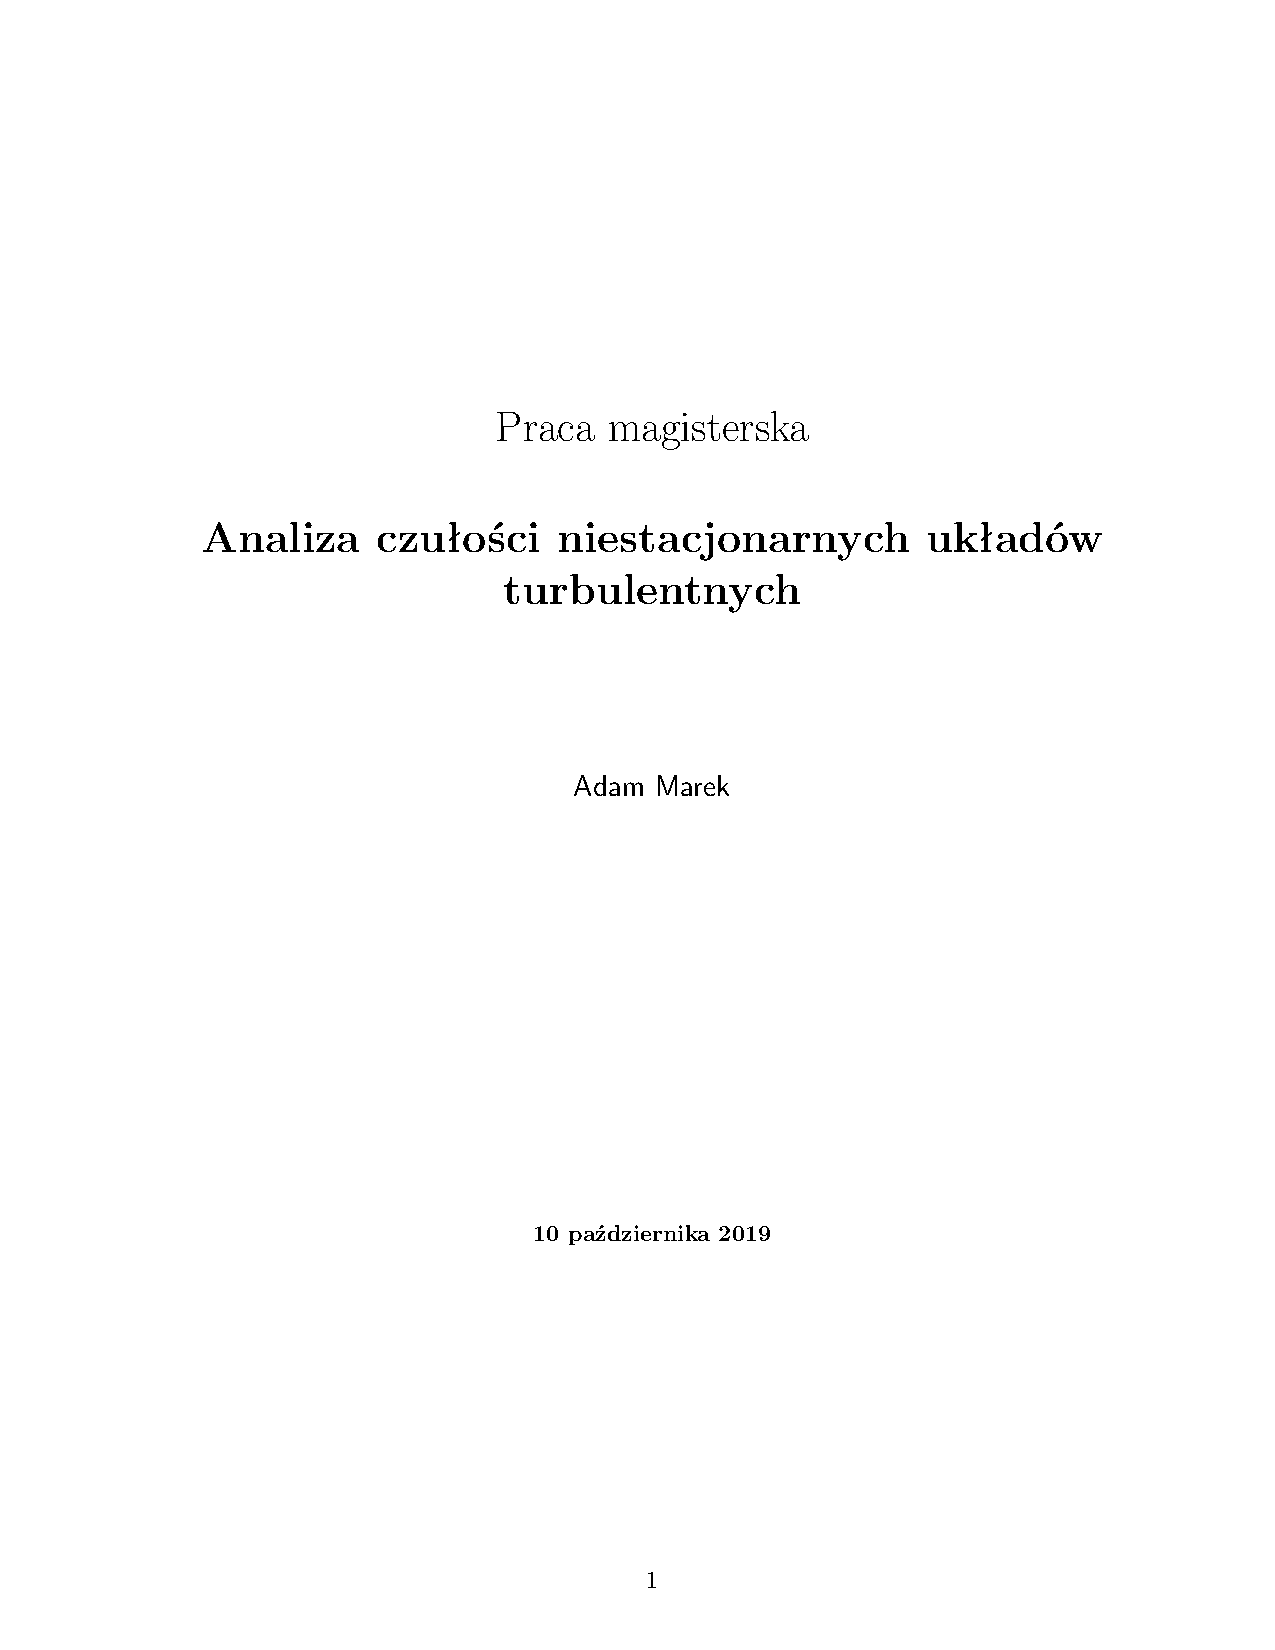
\includegraphics[scale=0.7]{figures/LSS.png} 
	\centering
	\caption{Czułość funkcji celu wyznaczona metodą trajektorii cienia.)}
\end{figure}
\begin{figure}[H]
	\includegraphics[scale=0.7]{figures/LSSvsCVM.png} 
	\centering
	\caption{Porównanie obu metod}
\end{figure}
Podobna analiza została wykonana dla drugiego przypadku ($ T=50 $), a jej wyniki przedstawiają Rysunki  oraz .
\begin{figure}[H]
	\includegraphics[scale=0.7]{figures/LSS1.png} 
	\centering
	\caption{Czułość funkcji celu wyznaczona metodą trajektorii cienia.)}
\end{figure}
\begin{figure}[H]
	\includegraphics[scale=0.7]{figures/LSSvsCVM1.png} 
	\centering
	\caption{Porównanie obu metod}
\end{figure}
Kod zaimplementowany w środowisku skryptowym MATLAB jest dostępny na publiczny repozytorium autora \cite{Marek1}.
\subsection{Scenariusz II - oblicze chaosu}
\subsubsection{Słowo wstępne}
Jak zostało zaznaczone na wstępie, głównym celem niniejszej pracy jest analiza wrażliwości wybranej funkcji celu dla zagadnienia przepływowego modelowanego równaniem Boltzmanna. Konkretniej: chcemy zastosować Metodę Trajektorii Cienia do zagadnienia rozwiązywanego Metodą Siatek Boltzmanna (ang. \textit{Lattice Boltzmann Method}). Istnieje cały szereg zalet nautry numerycznej, które pokrótce zostaną przedstawione w następnym podrozdziale. Jednak już w tym momencie należy wmienić obszary praktycznych zastosować, które wykorzystują wspomnianą metodę. Są to między innymi:
W poprzednim rozdziale została przedstawiona metoda LSS w sposób generyczny. Obecnie należy dopasować jej schemat w celu regularyzacji równań opisujących dynamikę rozważanego przepływu. W momencie pisania tej pracy autor nie spotkał się z żadną istniejącą implementacją tej metody dla zdyskretyzowanych równań Boltzmanna - znane są jedynie aplikacje dla solverów bazujących na równaniach Naviera-Stokesa. Należy przy tym dodatkowo zaznaczyć, że wszystkie one oparte są o przechowywanie powstałej macierzy układu równań w pamięci. W dalszej części pracy ukazane zostaną wady takiego podejścia (w szczególności, zajętość pamięci operacyjnej w takich przypadkach całkowicie niweluje, zdaniem autora, jakiekolwiek szanse na ich użycie w praktycznych zastosowaniach - nawet dla układów dwuwymiarowych korzystających z modeli turbulencji klasy RANS). Praca owa skupia się na podejściu, w którym macierz układu trajktuje się w sposób 'abstrakcyjny' - jako funktor, którego argumentami są wektory wejściowe, zaś wyjście stanowi iloczyn macierzy i wektorów wejściowych.
Do opisu implementacji Metody Trajektorii Cienia konieczna jest znajomośc równań wykorzystywanych w Metodzie Siatek Boltzmanna, dlatego też w dalszej części pracy skrótowo opisane zostały podstawowe jej założenia i płynące z nich wnioski w postaci gotowych formuł. Następnie zaprezentowane zostanły wyniki obliczeń dla przykładowego zagadnienia, w którym następuje oderwanie strugi na skutek skokowej zmiany geometrii. Zbadana zostanie przy tym czułość średniego spadku ciśnienia w długim horyzoncie czasowym w stosunku do modułu prędkości zadanej na wlocie do obszaru obliczeniowego.
\subsubsection{Metoda Siatek Boltzmanna}
Jak już zostało nieformalnie wspomniane (przy okazji omawiania pojęcia ergodyczności) w mechanice statystycznej definiuje się rokład prawdopodobieństwa związany z nazwiskami Boltzmanna oraz Maxwella. Ma on następującą postać
Podstawowym założeniem prowadzącym do takiej dystrybucji prędkości wśród cząstek jest przyjęcie modelu gazu doskonałego oraz założenie równowagi termodynamicznej między układem jego otoczeniem. Należy zwrócić uwagę na znaczenie tego rozkładu - jest to gęstość prawdopodobieństwa stanowiąca miarę liczności cząstek w danym zakresie prędkości. Jak każda funkcja gęstości prawdopodobieństwa jest ona równa prawie wszędzie pochodnej dystrybuanty związanej z tym rozkładem. Wobec tego, na poziomie intuicji, można taką funkcję utożsamiać ze stosunkiem liczby cząstek mających ograniczony zakres przyjmowanych prędkości w stosunku do całkowitej ich liczby. Zauważmy, że podejście to nie opisuje każdej cząstki jako oddzielnego składnika złożonego systemu (podejście mikroskopowe). Jednakże jest ono również odmienne od dobrze znanego z obecnie najpopularniejszych metod modelowania komputerowego przepływów uśredniania w relatywnie niewielkiej (w sensie rozciągłości przestrzennej) parametrów statystycznie istotnej liczby cząstek, z którego generowane są pola parametrow makroskopowych takich jak ciśnienie, temperatura czy prędkość (podejście to bazuje na założeniu ciągłości badanego ośrodka i nazywane jest podejściem makroskopowym). Głównym zamysłem Metody Siatek Boltzmanna jest symulowanie ewolucji w czasie analogicznego rozkładu (niekoniecznie dla stanów równowagowych).

\subsubsection{Model matematyczny}
Jako schemat połączeń węzłów siatki przyjęty został typ d2Q9 (Rysunek)
\begin{figure}[H]
	\includegraphics[scale=0.7]{figures/d2q9.jpg} 
	\centering
	\caption{Schemat połączeń węzłów siatki}
\end{figure}
W przyjętym modelu metody siatek Boltzmanna dyskretne równanie zadające dynamikę ma następującą postać:
\begin{equation}
f_{i}(x + \Delta x, t + \Delta t) = f_{i}(x,t) - \frac{1}{\tau_f}[f_{i}(x,t) - f_{i}^{eq}(x,t)].
\end{equation}
Przyjmujemy, że $f_{i}(x,t)$ oznacza funkcję rozkładu cząstek dla $i$-tej prędkości w punkcie $x$ w chwili $t$. Parametry siatki oznaczamy przez $\Delta x$ oraz $\Delta t$, zaś $\tau_f$ jest charakterystycznym czasem relaksacji.
Jeśli pozostawimy układ bez wpływu czynników zewnętrznych, będzie on dążył do stanu równowagi, dla której równowagowa funkcja gęstości rozkładu $f^{eq}$, która ma postać:
\begin{equation}
f_{i}^{eq} = \rho w_{i} \Bigg[1 + \frac{e_i \cdot u}{c_{s}^{2}} + 
\frac{(e_i \cdot u)^2 - (c_s|u|)^2}{2 c_{s}^{2}}\Bigg],
\end{equation}
gdzie $w_0 = \frac{4}{9}$, $w_{1,2,3,4} = \frac{1}{9}$, $w_{5,6,7,8} = \frac{1}{36}$, $c_s = \sqrt{3}c$, gdzie $c = \frac{\Delta x}{\Delta t}$, przy czym $c_s$ interpretujemy jako prędkość dźwięku w płynie. Prędkość $u$ wyraża się wzorem:
\begin{equation}
u = \sum_{i=0}^{8}f_{i}e_{i},
\end{equation}
gdzie prędkości w kierunku $i$ są postaci:
\begin{equation}
e_i = \left\{ \begin{array}{ll}
(0,0)c & \textrm{gdy $i = 0$}\\
(\cos[(i-1)\frac{\pi}{2}], \sin[(i-1)\frac{\pi}{2}])c & \textrm{gdy $i=1,2,3,4$}\\
(\sqrt{2}\cos[(2i-9)\frac{\pi}{4}],\sqrt{2}\sin[(2i-9)\frac{\pi}{4}])c & \textrm{gdy $ i=5,6,7,8 $}
\end{array} \right.
\end{equation}
Gęstość w punkcie $x$ w chwili $t$ jest postaci:
\begin{equation}
\rho(x,t) = \sum_{i=0}^{8}f_{i}(x,t).
\end{equation}
Dodatkowo, gdy na cząsteczki działa zewnętrzna siła $F$, to makroskopowa prędkość płynu wyraża się następująco:
\begin{equation}
U(x,t) = u(x,t) + \frac{1}{2}\frac{F(x,t)}{\rho(x,t)}.
\end{equation}
Dynamika w podejściu tej metody modelowana jest zatem dwustopniowo: pierwszy etap stanowi kolizja (reprezentowana operatorem kolizji), drugi zaś stanowi propagację funkcji rozkładu zgodnie z dyskretnymi kierunkami wybranych wektorów prędkości. W pracy operator kolizji jest aproksymowany dobrze rozpoznanym modelem BGK. Należy zwrócić uwagę, iż rozkład równowagowy jest wielomianowym przybliżeniem rozkładu Maxwella-Boltzmanna.\newline
Kształt obszaru obliczeniowego został zilustrowany na Rysunku
Pomimo tak prostej geometrii w przepływie takim występuje szereg zjawisk o skomplikowanej naturze:
\begin{itemize}
	\item niestabilność przepływu
	\item przejście laminarno-turbulentne
	\item separacja warstwy przyściennej
	\item oderwanie warstwy przyściennej
	\item recyrkulacja,
\end{itemize}
wobec czego przypadek ten często traktywany jest jako sprawdzian testowy dla różnych modeli turbulencji \cite{Salazar}.
\subsubsection{Aspekty numeryczne}
Zanim przejdziemy do omówienia wyników należy chwilę poświęcić na aspekty implementacyjne, gdyż dla zagadnień wielowymiarowych odgrywają one kluczową rolę. W typowych przypadkach przepływów mogą nawet zadecydować o możliwości wykorzystania danej metody.
\subsubsection{Wyniki symulacji - pierwsze podejście}
Geometrię obszaru obliczeniowego przedstawia Rysunek
\begin{figure}[H]
	\includegraphics[scale=1.8]{figures/geometry.png} 
	\centering
	\caption{Geometria obszaru obliczeniowego}
\end{figure}
W rozważanym przypadku $ H = 2 $, $ h_{i}=h=L_{i}=1 $ oraz $ L_{c}=9 $.\newline
Jako funkcję celu przyjęty został średni spadek ciśnienia między wlotem a wylotem, zaś jako parametr kontrolny przyjęty został moduł prędkości wlotowej (przyjęty został tłokowy rozkład prędkości na wlocie):
\begin{equation}
\bar{J} = \frac{1}{T}\int_{0}^{T}(\hat{p}_{in}(t)-\hat{p}_{out}(t))dt,
\end{equation}
gdzie $ \hat{p}_{in}(t) $ oraz $ \hat{p}_{out}(t) $ oznaczają średnie ciśnienie w chwili $ t $ na wlocie oraz wylocie, odpowiednio. Funkcja ta dla badanej geometrii w przypadku różnych prędkości $ u \in [0.05 ; 0.15]$ na wlocie została zilustrowana na Rysunku.
\begin{figure}[H]
	\includegraphics[scale=0.7]{figures/Jbar.png} 
	\centering
	\caption{Wartość funkcji celu w zależności od parametru kontrolnego}
\end{figure}
Zależność ta ma kształt paraboliczny, co jest zgodne z oczekiwaniami. Uwagę tę potwierdza Rysunek, który ilustruje krzywą na tle najlepiej dopasowanej doń paraboli.
Przebadane zostały trzy przypadki różniące się liczbą Reynoldsa (modułem prędkości wlotowej). Rozmiary siatki pozostawały niezmienne.
\paragraph{Liczba Reynoldsa: 200}
Rysunki przedstawiają mapy modułu prędkości po 1000, 2000, 3000 oraz 4000 kroków czasowych, odpowiednio (rysunki zostały odpowiednio przeskalowane w kierunku osi pionowej dla przejrzystości poglądu).
\begin{figure}[H]
	\includegraphics[scale=0.3]{figures/LBM/u0_05_1.png} 
	\caption{Mapa modułu prędkości po $ T=1000 $ kroków czasowych}
\end{figure}
\begin{figure}[H]
	\includegraphics[scale=0.3]{figures/LBM/u0_05_2.png} 
	\caption{Mapa modułu prędkości po $ T=2000 $ kroków czasowych}
\end{figure}
\begin{figure}[H]
	\includegraphics[scale=0.3]{figures/LBM/u0_05_3.png} 
	\caption{Mapa modułu prędkości po $ T=3000 $ kroków czasowych}
\end{figure}
\begin{figure}[H]
	\includegraphics[scale=0.3]{figures/LBM/u0_05_4.png} 
	\caption{Mapa modułu prędkości po $ T=4000 $ kroków czasowych}
\end{figure}
\paragraph{Liczba Reynoldsa: 400}
Rysunki przedstawiają mapy modułu prędkości po 1000, 2000, 3000 oraz 4000 kroków czasowych, odpowiednio 
\begin{figure}[H]
	\includegraphics[scale=0.3]{figures/LBM/u0_10_1.png} 
	\caption{Mapa modułu prędkości po $ T=1000 $ kroków czasowych}
\end{figure}
\begin{figure}[H]
	\includegraphics[scale=0.3]{figures/LBM/u0_10_2.png} 
	\caption{Mapa modułu prędkości po $ T=2000 $ kroków czasowych}
\end{figure}
\begin{figure}[H]
	\includegraphics[scale=0.3]{figures/LBM/u0_10_3.png} 
	\caption{Mapa modułu prędkości po $ T=3000 $ kroków czasowych}
\end{figure}
\begin{figure}[H]
	\includegraphics[scale=0.3]{figures/LBM/u0_10_4.png} 
	\caption{Mapa modułu prędkości po $ T=4000 $ kroków czasowych}
\end{figure}
\paragraph{Liczba Reynoldsa: 600}
Rysunki przedstawiają mapy modułu prędkości po 1000, 2000, 3000 oraz 4000 kroków czasowych, odpowiednio 
\begin{figure}[H]
	\includegraphics[scale=0.3]{figures/LBM/u0_15_1.png} 
	\caption{Mapa modułu prędkości po $ T=1000 $ kroków czasowych}
\end{figure}
\begin{figure}[H]
	\includegraphics[scale=0.3]{figures/LBM/u0_15_2.png} 
	\caption{Mapa modułu prędkości po $ T=2000 $ kroków czasowych}
\end{figure}
\begin{figure}[H]
	\includegraphics[scale=0.3]{figures/LBM/u0_15_3.png} 
	\caption{Mapa modułu prędkości po $ T=3000 $ kroków czasowych}
\end{figure}
\begin{figure}[H]
	\includegraphics[scale=0.3]{figures/LBM/u0_15_4.png} 
	\caption{Mapa modułu prędkości po $ T=4000 $ kroków czasowych}
\end{figure}
Kod zaimplementowany w języku C++ jest dostępny na publiczny repozytorium autora \cite{Marek2}.
\newpage
\begin{thebibliography}{99}
\bibitem{Blonigan1} Blonigan P. J., Wang Q.,
\emph{Probability density adjoint for sensitivity analysis of the mean chaos},
Journal of Computational Physics, 235 (2014) 1-13.

\bibitem{Blonigan2} Blonigan P. J., Wang Q., Nielsen E. J., Diskin B.,
\emph{Least Squares Shadowing sensitivity analysis of chaotic flow around a tw-dimensional airfoil},
in: 54th AIAA Aerosoace Sciences Meeting, January 2016, pp. 1-28.

\bibitem{Blonigan3} Blonigan P. J., Wang Q.,
\emph{Least Squares Shadowing sensitivity analysis of a modified Kuramoto-Sivashinsky eqation},
Chaos Solitons Fractals, 64, 2014, 16-25.

\bibitem{Chandramoorthy} Chandramoorthy, N., Fernandez, P., Talnikar, C., Wang, Q. 2017 
\emph{An Analysis of the Ensemble Adjoint Approach to Sensitivity Analysis in Chaotic Systems} 
AIAA Paper 2017-3799. 

\bibitem{Evans} Evans L.C.,
\emph{Równania różniczkowe cząstkowe},
Wydawnictwo: PWN, Warszawa 2012.

\bibitem{Gleick} Gleick J.,
\emph{Chaos. Narodziny nowej nauki.},
Wydawnictwo: Zysk i S-ka, 2018.

\bibitem{Golub} Golub G. H., Loan C. V. F.,
\emph{Matrix Computations},
The Johns Hopkins Univ. Press, Baltimore, 1996.

\bibitem{Kudrewicz} Kudrewicz J., 
\emph{Fraktale i chaos},
Wydawnictwo: WNT, 1996.

\bibitem{Lea1} Lea D., Allen M., Haine T.,
\emph{Sensitivity analysis of the climate of a chaotic system},
Tellus, Vol. 52A, 2000, pp. 523-532.

\bibitem{Lea2} Lea D., Haine T., Allen M., Hansen J., 
\emph{Sensitivity analysis of the climate of a chaotic ocean circulation model},
Journal of the Royal Meteorological Society, Vol. 128, 2002, pp. 2587-2605.

\bibitem{Lorenz} Lorenz E.,
\emph{Deterministic Nonperiodic Flow},
Journal of Atmospheric Sciences, Vol. 20, 1963, pp. 130-141.

\bibitem{Marek1} Marek A.,
\emph{ChaoticSystemsOptimization},
https://github.com/BlooAM/ChaoticSystemsOptimization, 2019.

\bibitem{Marek2} Marek A.,
\emph{LSS},
https://github.com/BlooAM/LSS, 2019.

\bibitem{Maurin1} Maurin K.,
\emph{Analiza, część I},
Wydawnictwo: PWN, Warszawa 2010.

\bibitem{Maurin2} Maurin K.,
\emph{Analiza, część II},
Wydawnictwo: PWN, Warszawa 2010.

\bibitem{Maurin3} Maurin K.,
\emph{Analiza, część III},
Wydawnictwo: PWN, Warszawa 2010.

\bibitem{Palczewski} Palczewski A.,
\emph{Równania różniczkowe zwyczajne. Teoria i metody numeryczne z wykorzystaniem programu rachunków symbolicznych},
Wydawnictwo: WNT, Warszawa 2017.

\bibitem{Ruelle1} Ruelle D.,
\emph{Differentiation of SRB states},
Communications in Mathematical Physics, Vol. 187, 1997, pp. 227-241.

\bibitem{Ruelle2} Ruelle D.,
\emph{ A review of linear response theory for general differentiable dynamical systems},
Nonlinearity 22 (4) (2009) 855.

\bibitem{Salazar} Salazar J., Santos L.
\emph{2d lattice-boltzmann simulations of flow over a backward-facing step at low to moderate reynolds numbers},
GRAD - Fluid Physics and Transport Phenomena Research Group, Universidade Federal deSanta Catarina
	
\bibitem{Strogatz} Strogatz S., 
\emph{Nonlinear Dynamics and Chaos: With Applications to Physics, Biology, Chemistry and Engineering},
Westview Press, Philadelphia, PA, 1994.  

\bibitem{Tempczyk} Tempczyk M., 
\emph{Teoria chaosu dla odważnych},
Wydawnictwo: PWN, Warszawa 2002.
	
\bibitem{Qiqi1} Wang Q.,
\emph{Forward and adjoint sensitivity computation of chaotic dynamical systems},
Journal of Computational Physics, 235 (2013) 1-13.

\bibitem{Qiqi2} Wang Q.,
\emph{Convergence of the Least Squares Shadowing Method for Computing Derivative of Ergodic Averages},
SIAM Journal of Numerical Analysis, Vol 52, No. 1, 2014, pp. 156-170.  

\bibitem{Qiqi3} Wang Q., 
\emph{Least Squares Shadowing sensitivity analysis of chaotic limit cycle oscillations},
Journal of Computational Physics, Vol. 267, June 2014, pp. 210-224.  

\bibitem{Encyclopedie}
\emph{https://plato.stanford.edu/entries/chaos/},
\end{thebibliography} 
\end{document}

%%%%%%%%%%%%%%%%%%%%%%%%%%%%%%%%%%%%%%%%%%%%%%%%%%%%%%%%%%%%%%%%%%%%%%%
%%%%%%%%%%%%%%%%%%%%%%%%%%%%%%%%%%%%%%%%%%%%%%%%%%%%%%%%%%%%%%%%%%%%%%%